\documentclass[12pt, letterpaper]{article}
\usepackage[
    backend=biber,
    style=numeric,
]{biblatex} 
\usepackage{graphicx}
\usepackage{enumitem}
\usepackage{pdfpages}
\usepackage{listings, listings-rust}
\usepackage[utf8]{inputenc}
\usepackage[acronym]{glossaries}

\graphicspath{{diagrams/}}
\addbibresource{sources.bib}

\title{
    \Huge \textbf{Software-Implemented Fault Tolerance}
}
\author{Filip Ďuriš}

\definecolor{codegreen}{rgb}{0,0.6,0}
\definecolor{codegray}{rgb}{0.4,0.4,0.4}
\definecolor{codepurple}{rgb}{0.58,0,0.82}
\definecolor{backcolour}{rgb}{1,1,1}

\lstdefinestyle{mystyle}{
    backgroundcolor=\color{backcolour},   
    commentstyle=\color{codegreen},
    keywordstyle=\color{magenta},
    numberstyle=\tiny\color{codegray},
    stringstyle=\color{codepurple},
    basicstyle=\ttfamily\footnotesize,
    breakatwhitespace=false,         
    breaklines=true,                 
    captionpos=b,                    
    keepspaces=true,                 
    numbers=left,                    
    numbersep=5pt,                  
    showspaces=false,                
    showstringspaces=false,
    showtabs=false,                  
    tabsize=2
}

\lstset{style=mystyle}

% SETTINGS - NAMES
\newcommand{\myTitle}[0] {Software-implemented fault tolerance}
\newcommand{\myName}[0] {Filip Ďuriš}
\newcommand{\mySupervisor}[0] {Ing. Ján Mach}
\newcommand{\myEvidenceNumber}[0] {FIIT-100241-117028}
\newcommand{\myDate}[0] {Máj 2025}
\newcommand{\myStudyProgram}[0] {Informatics}
\newcommand{\myDegreeCourse}[0] {9.2.5 Software Engineering}
\newcommand{\myInstitute}[0] {Institute of Informatics and Software Engineering, FIIT STU, Bratislava}
\newcommand{\FIITuniversity}[0] {Slovak University of Technology in Bratislava}
\newcommand{\FIITuniversitySK}[0] {Slovenská technická univerzita v Bratislave}
\newcommand{\FIITfaculty}[0] {Faculty of informatics and information technologies}
\newcommand{\FIITfacultySK}[0] {Fakulta informatiky a informačných technológií}
\newcommand{\FIITthesis}[0] {Bachelor's thesis}
\newcommand{\FIITthesisSK}[0] {Bakalárska práca}
\newcommand{\FIITstudyProgram}[0] {Informatics}
\newcommand{\FIITstudyProgramSK}[0] {Informačná bezpečnosť}
\newcommand{\FIITstudyField}[0] {Computer Science}
\newcommand{\FIITdegreeCourseSK}[0] {9.2.1 Informatika}
\newcommand{\FIITinstitute}[0] {Institute of Informatics, Information Systems and Software Engineering}
\newcommand{\FIITinstituteSK}[0] {Ústav informatiky, informačných systémov a softvérového inžinierstva}

\makeglossaries

\newacronym{gcd}{GCD}{Greatest Common Divisor}

\newacronym{lcm}{LCM}{Least Common Multiple}

\begin{document}

% % Cover page
\begin{center}
\thispagestyle{empty}
{\Large \FIITuniversity}
\par\end{center}{\Large \par}

\begin{center}
{\Large \FIITfaculty}
\par\end{center}{\Large \par}

\smallskip{}

\begin{center}
Reg. No.: \myEvidenceNumber
\par\end{center}
\vfill{}

\begin{center}
\textbf{\Large \myTitle}
\par\end{center}{\Large \par}

\medskip{}


\begin{center}
\textbf{\LARGE \myTitle}
\par\end{center}{\huge \par}

\medskip{}


\begin{center}

{\Large \FIITthesis}
\par\end{center}{\Large \par}

\vfill{}

Thesis supervisor: \mySupervisor


\medskip{}

\myDate

\pagenumbering{roman}

\clearpage



% Thesis title page
\begin{center}
\thispagestyle{empty}
{\Large \FIITuniversity}
\par\end{center}{\Large \par}

\begin{center}
{\Large \FIITfaculty}
\par\end{center}{\Large \par}

\smallskip{}

\begin{center}
Reg. No.: \myEvidenceNumber
\par\end{center}
\vfill{}

\begin{center}
\textbf{\Large \myTitle}
\par\end{center}{\Large \par}

\medskip{}


\begin{center}
\textbf{\LARGE \myTitle}
\par\end{center}{\huge \par}

\medskip{}


\begin{center}

{\Large \FIITthesis}
\par\end{center}{\Large \par}

\vfill{}

Study programme: \FIITstudyProgram

Study field: \FIITstudyField

Training workplace: \FIITinstitute

Thesis supervisor: \mySupervisor

\medskip{}

\myDate

\clearpage


% \newpage


\includepdf[pages={1}]{front_page.pdf}
\newpage


\includepdf[pages={1}]{assignment.pdf}
\newpage

\thispagestyle{empty}

\newcommand{\signaturespace}[2]{
  % #1 = width of the dotted line
  % #2 = legend
  \begingroup
  \renewcommand{\arraystretch}{0}
  \begin{tabular}[t]{cc}
  \hspace*{0pt}
  \cleaders\hbox{\kern.6pt.\kern.6pt}\hskip#1\relax
  \hspace*{0pt}
  \\[0.5cm]
  #2
  \end{tabular}
  \endgroup
}

\vspace*{\fill}


I declare on my honor that I have prepared this work independently, on the basis of consultations and using the listed literature. \\

In Bratislava 12.5.2025
\hspace*{\fill} \signaturespace{5cm}{\myName}


\clearpage


\thispagestyle{empty}

\section*{Annotation}

\begin{minipage}[t]{1\columnwidth}%
Slovak University of Technology Bratislava 

Faculty of Informatics and Information Technologies

Degree Course: \myStudyProgram\\

Author: \myName

Bachelor's Thesis: \myTitle

Supervisor: \mySupervisor

\myDate%
\end{minipage}

\bigskip{}

This thesis explores software-implemented fault tolerance for embedded systems, with a particular focus on solutions that do not require specialized or redundant hardware. As embedded systems grow increasingly complex and are deployed in harsher or more unpredictable environments, the risk of system failure rises accordingly. Traditional approaches to fault tolerance often rely on hardware redundancy, such as error-correcting memory or replicated components, which significantly increases development cost, power consumption, and physical space requirements. In contrast, this research investigates software-only techniques that can detect, mitigate, or recover from faults without the need for specialized hardware. The study examines various software fault-tolerance techniques and evaluates their trade-offs in terms of reliability, performance overhead, and implementation complexity. A practical case study is presented using the Rust programming language and the FreeRTOS real-time operating system on a RISC-V embedded platform. Through empirical testing of selected techniques under simulated fault conditions, the findings demonstrate that software-based fault tolerance can provide a meaningful level of protection, particularly for non-critical applications.

\thispagestyle{empty}
\mbox{}
\newpage

\thispagestyle{empty}
\section*{Anotácia}

\begin{minipage}[t]{1\columnwidth}%
Slovenská technická univerzita v Bratislave

Fakulta informatiky a informačných technológií

Študijný program: \myStudyProgram\\

Autor: \myName

Bakalárska práca: \myTitle

Vedúci bakalárskej práce: \mySupervisor

\myDate%
\end{minipage}

\bigskip{}

Táto bakalárska práca sa zaoberá softvérovo implementovanou odolnosťou voči poruchám vo vstavaných systémoch, so zvláštnym zameraním na riešenia, ktoré nevyžadujú špecializovaný alebo redundantný hardvér. S rastúcou zložitosťou zabudovaných systémov a ich nasadzovaním v náročnejších a menej predvídateľných prostrediach sa zvyšuje aj riziko zlyhania systému. Tradičné prístupy k odolnosti voči poruchám sa často spoliehajú na hardvérovú redundanciu, ako sú pamäte s korekciou chýb alebo duplikované komponenty, čo výrazne zvyšuje náklady na vývoj, spotrebu energie a nároky na fyzický priestor.

Táto práca skúma výlučne softvérové techniky, ktoré dokážu poruchy detegovať, zmierniť ich dopad alebo sa z nich zotaviť bez potreby špecializovaného hardvéru. Štúdia analyzuje rôzne softvérové prístupy k zabezpečeniu odolnosti voči poruchám a hodnotí ich kompromisy z hľadiska spoľahlivosti, výkonnostnej záťaže a zložitosti implementácie. Praktická demonštrácia využíva programovací jazyk Rust a real-time operačný systém FreeRTOS na platforme RISC-V. Pomocou empirických testov vybraných techník v simulovaných poruchových podmienkach práca ukazuje, že softvérovo implementovaná odolnosť voči poruchám môže poskytnúť zmysluplnú úroveň ochrany, najmä pre nekritické aplikácie.

\clearpage




\tableofcontents
\newpage

Given a set of numbers, there are elementary methods to compute 
its \acrlong{gcd}, which is abbreviated \acrshort{gcd}. This process 
is similar to that used for the \acrfull{lcm}.

\glsaddall
\printglossary[type=\acronymtype]
% \printglossary

\section{Introduction}

% \begin{abstract}
With the increasing demand for high-performance embedded software comes the inevitable, difficult task of ensuring fault-free functioning of ever-more complex systems. The increased complexity, both in terms of hardware components and software features, increases the number of failure points where errors can manifest.

Errors can be caused by both external factors beyond our control such as radiation in space, but also as a result of human error while designing the software. Due to the incredibly complex nature of this problem, it is unlikely that we will be designing completely error-free software and hardware in the near future. This makes fault-tolerance an important aspect of software design, especially when designing critical systems whose failure could endanger human life. However, as with most things, fault-tolerance and reliability is a trade-off, which usually comes at the cost of performance and development time.

Historically, specialized hardware was the go-to choice for implementing fault tolerance, specifically by hardening and or duplicating the components. This approach requires designing and producing non-standard computer components, exponentially increasing the development cost. Lately, a more economical solution began gaining traction for non-critical missions. Namely, using off-the-shelf components without specialized hardening, while using software redundancies to implement fault tolerance.

This thesis will aim to analyze various common software-implemented fault-tolerance methods. We will look at the benefits and drawbacks of the utilized methods, as well as construct a working demo based on FreeRTOS running on RISC-V core that implements and tests the effectiveness of some selected methods using the Rust programming language.
% \end{abstract}

\newpage

\section{Nomenclature}

For the sake of consistency in the terms used in this document, we will refer to the naming conventions and definitions as outlined in \cite{1335465}. Below are the definitions of the most crucial terms used. \\

\textbf{Failure} is an event that occurs when the delivered service deviates from correct service. A service fails either because it does not comply with the functional specification, or because this specification did not adequately describe the system function. A service failure is a transition from correct service to incorrect service, i.e., to not implementing the system function \cite{1335465}.
\textit{Example: An I/O component not communicating with the system.} \\

\textbf{Failure domain}

\textbf{Fault} is the actual or hypothesized cause of an error. Faults are usually considered dormant until manifested, causing an error \cite{1335465}. An example of a fault might be hardware issue causing an I/O device to send corrupted data as input. If the software is not designed to deal with incorrect input this would lead to an internal error, possibly causing a service failure.
\textit{Example: A bit-flip in memory caused by radiation.} \\

\textbf{Error} is a deviation of the service from its correct state. It is a part of the system's state that may lead to service failure \cite{1335465}. Errors are the observable result of issues within the software and or hardware. 
\textit{Example: A fault that changes the output variable's value.} \\

\textbf{Fault Tolerance} is the system's ability to continue operating correctly in the presence of faults. Rather than eliminating faults entirely, fault-tolerant systems are designed to detect, isolate, and recover from faults before they cause service failures. 
\textit{Example: System operating correctly with one of its sensors not reponding.}\\

\textbf{System} is the collection of all components required to execute our program. This includes the processor with all of its components as well as any I/O peripherals and sensors, but also the program code.
\textit{Example: A microprocessor with a thermometer and antenna for communication.} \\

\textbf{System boundary} defines what is considered part of the system and what is not. It can be thought of as an imaginary line separating the components that make up the system from the outside world. Everything within the system boundary is part of the system, while everything outside is part of the environment.

\textbf{Service degradation} is the process of delivering incomplete or less optimal but still acceptable service. An example could be lowering video quality. 



\clearpage
\section{Requirements Specification}

The primary objective of this project is to analyze, implement, and evaluate selected software-based fault tolerance techniques. The focus is on embedded systems operating in environments where faults, particularly single event upsets (SEUs), can compromise system behavior. These issues are especially relevant in resource-constrained systems where safety and reliability are paramount, such as the aerospace or the automotive industry.

This section outlines the functional and non-functional requirements that the proposed system must fulfill to meet its objectives. The requirements are derived from practical scenarios and target use cases involving typical embedded workloads, including mathematical computations, sorting algorithms, and data integrity verification. These tasks will be executed under both normal and fault-injected conditions to evaluate the system's behavior and robustness.

\subsection*{Functional Requirements}
\begin{itemize}
\item The system shall implement multiple software-based fault tolerance techniques.
\item The system shall be capable of detecting and reporting transient faults at runtime.
\item The system shall provide a mechanism for recovering from detected faults where applicable (e.g., via checkpoint rollback or redundant execution).
\end{itemize}

\subsection*{Non-Functional Requirements}
\begin{itemize}
\item The system shall introduce minimal performance overhead relative to the unprotected baseline.
\item The solution shall be implemented entirely in software.
\item All fault tolerance methods shall be implemented in the Rust programming language to leverage its memory safety guarantees and low-level control.
\item The system shall be portable and capable of running on a 32-bit RISC-V platform using the FreeRTOS operating system.
\item The implementation shall be maintainable and modular, enabling future extension or substitution of fault tolerance mechanisms.
\end{itemize}

Ultimately, the project aims to deliver a practical and reproducible evaluation framework for software-based fault tolerance, enabling developers to assess the trade-offs between fault tolerance, runtime overhead, and system complexity in embedded contexts.
\newpage

\section{Types of faults}

In order to be able to analyze fault-tolerance techniques, we first need to understand the various types of faults that we might encounter. This list is not exhaustive and only covers fault types relevant to this thesis, for more complete list see \cite{1335465}. It is also important to understand two different classifications are not always mutually exclusive. As we will see later on, a solid fault, for example, can be caused during development, but can also be a product of external factors.

Faults can be further split into various categories, the ones mostly relevant to us are \textbf{external faults} which originate from outside the system boundaries and propagate into the system. Which also includes \textbf{natural faults} that are caused by natural phenomena without human participation. These faults can affect the hardware and the software, which is why we can further classify them as \textbf{hardware faults} and \textbf{software faults} respectively \cite{1335465}. \\

\subsection{Transient fault} is a temporary fault which results in an error. Transient faults are usually caused by random, external events (e.g. radiation) interfering with the system. A key characteristic of transient faults is the inability to accurately reproduce it, since the cause is external to the system. Retrying the same process multiple times is usually enough to deal with a transient fault, since it is extremely unlikely a transient fault will occur repeatedly within the same process at successive time intervals. If a fault persists across multiple attempts, it is possible we are dealing with a permanent fault. \\

\subsection{Permanent fault} also known as solid fault, is a lasting fault within the system that requires maintenance to remove. This could come in various forms, such as damaged hardware, corrupted memory or missing code. When dealing with a solid fault, retrying the same process is usually not enough as the same error will keep reoccurring. This approach requires alternatives and fallbacks within the system, which is outlined in more detail in section \ref{multi}. \\

\subsection{Hardware faults}

Hardware errors are caused by external factors beyond our control as software developers. They are usually caused by environmental influences, such as cosmic radiation in space, electro-magnetic fields or adverse weather conditions.

One of the most common hardware errors is memory corruption, which can appear in many forms and result from a wide range of causes. For instance, radiation exposure in space can cause SEUs, flipping individual bits in memory and altering data unpredictably. Similarly, physical damage to storage media, such as hard drives or SSDs, might corrupt specific regions of the file system, making certain data inaccessible or incorrect.

% Memory corruption is not always catastrophic. While it can result in complete system failure and unrecoverable states, it is just as likely to manifest as small, hard-to-detect errors. These subtle corruptions might not immediately disrupt the software's functioning but can lead to unpredictable behavior over time.

\begin{figure}[!hbt]
    \centering
    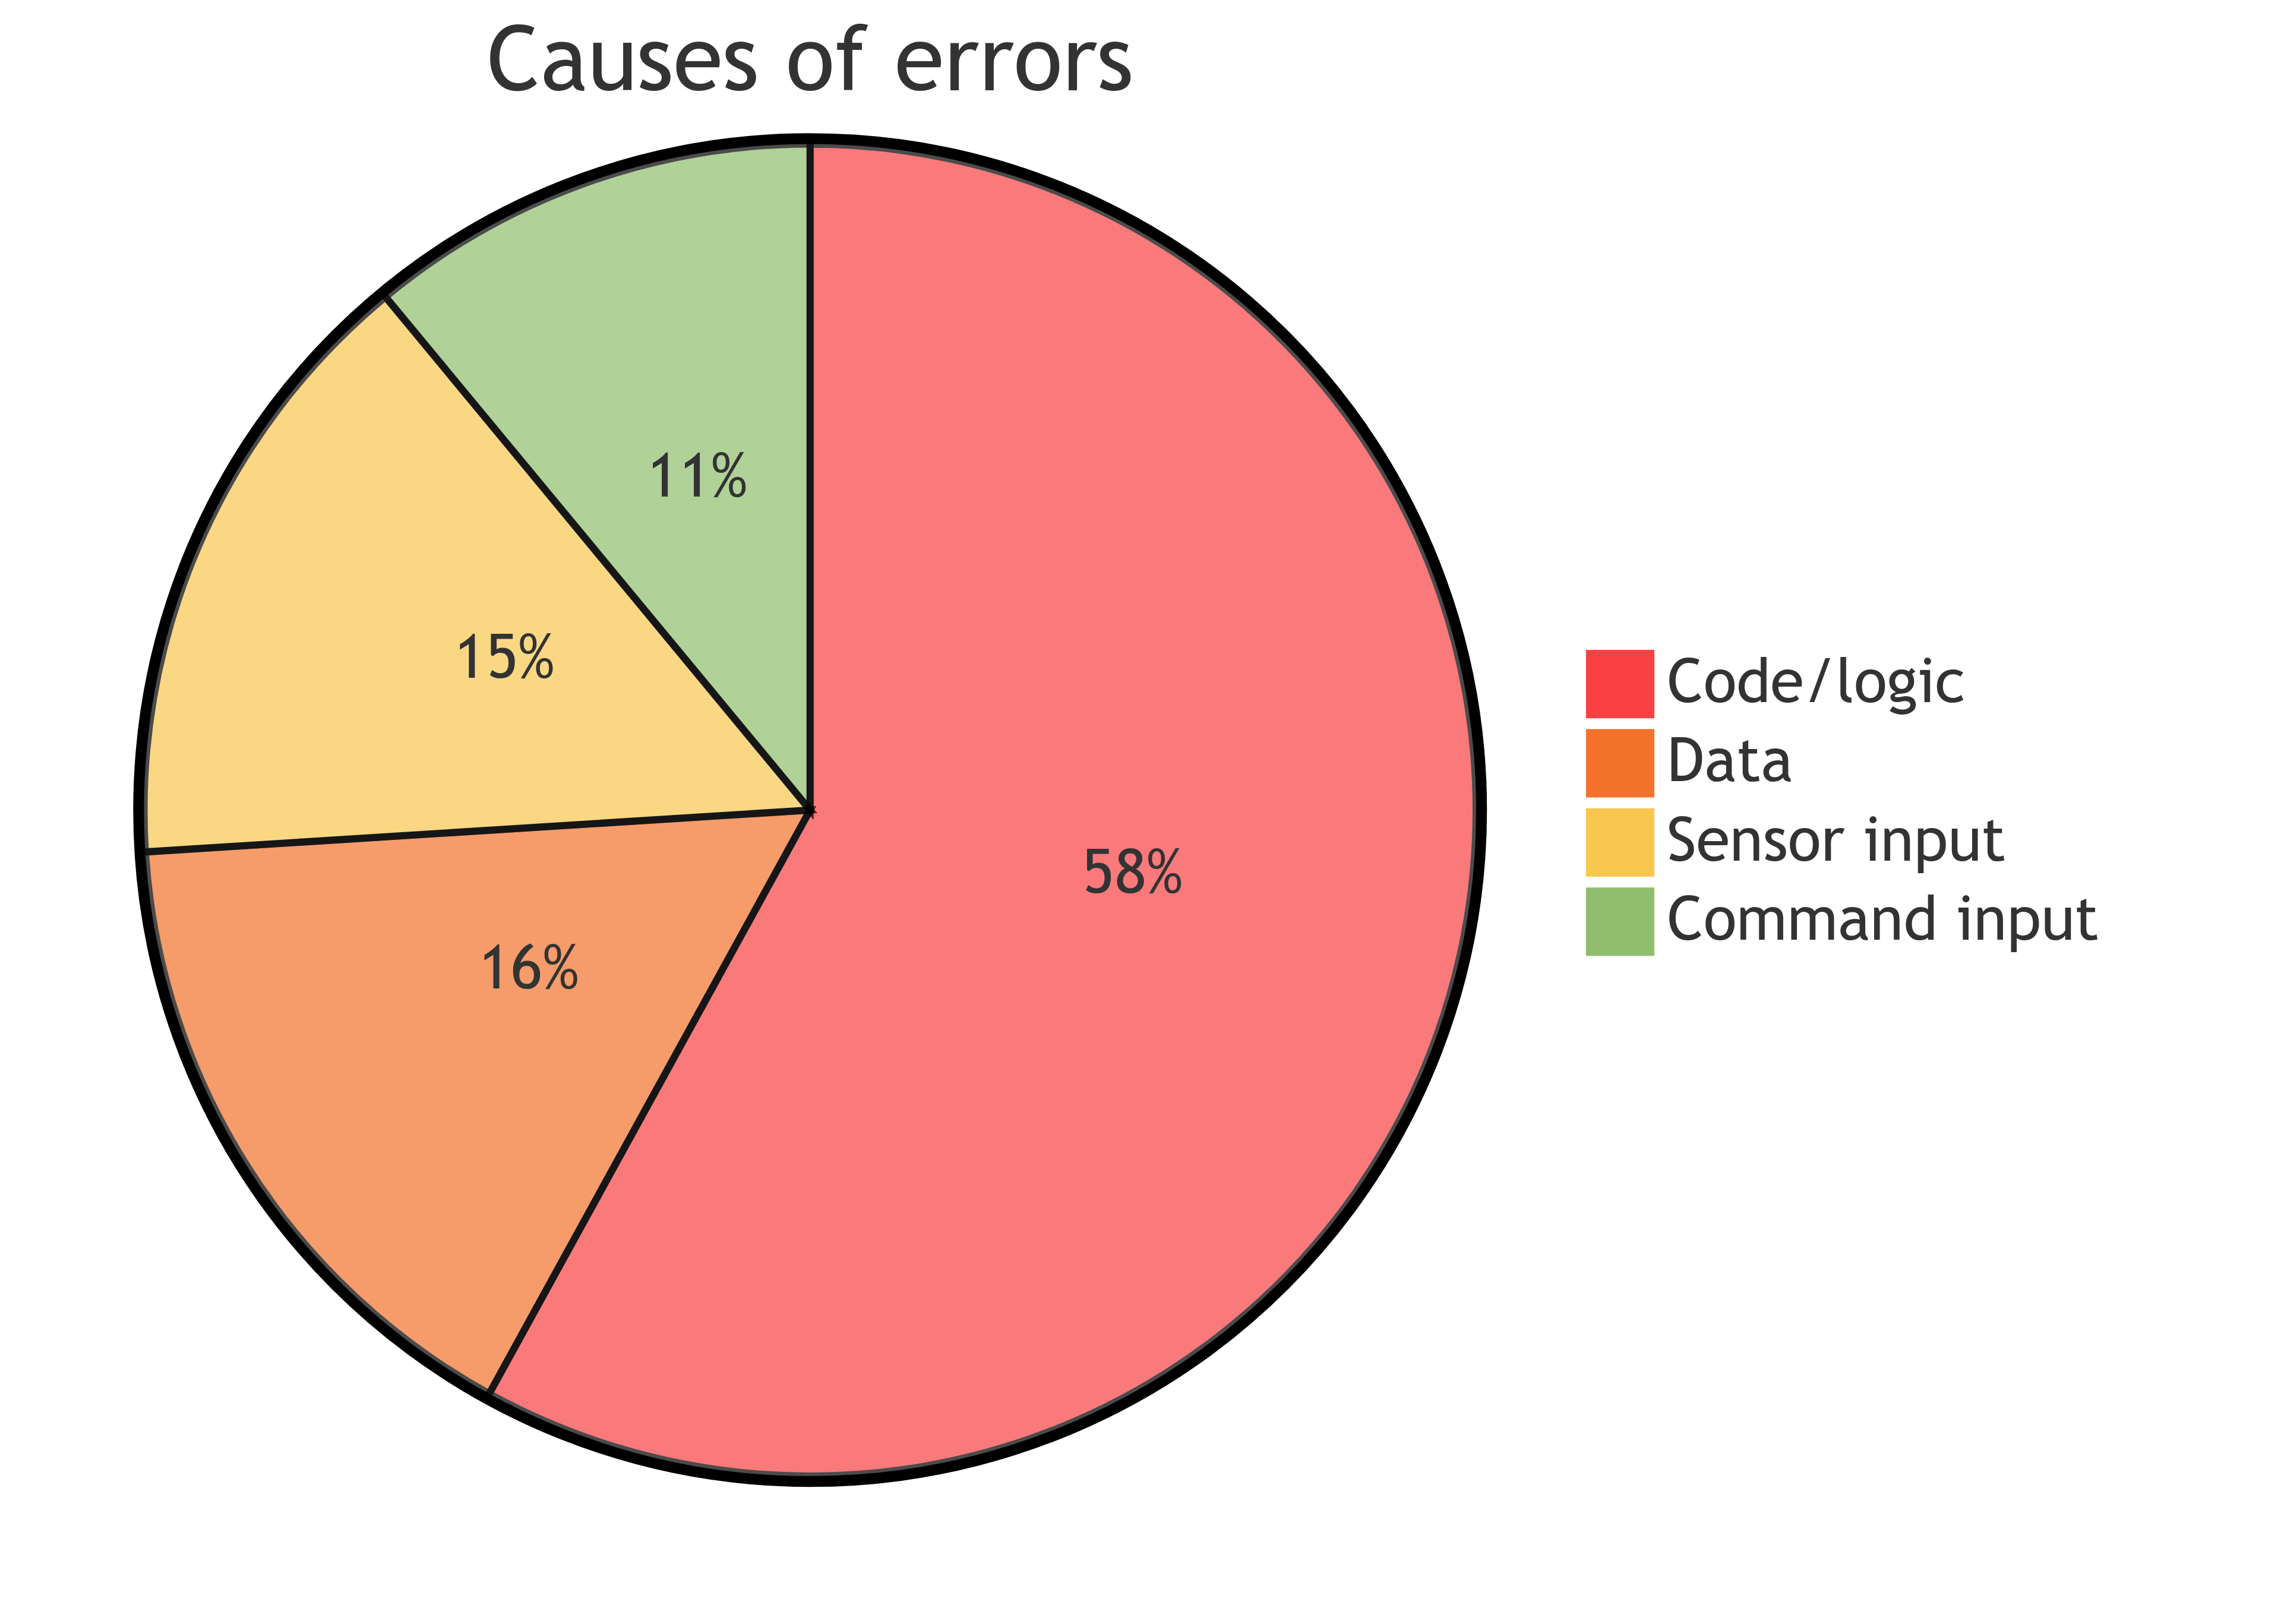
\includegraphics[width=0.6\textwidth]{diagrams/stats/piechart.png}
    \caption{Causes of errors \cite{nasa:stats}}
    \label{fig:nasa_stats}
\end{figure}

\subsection{Development faults}

Development faults is a category which includes all the various faults whose causes are introduced during software development stage. According to research conducted by NASA, majority of errors stem from faults within the code and logic of the afflicted software, followed closely by faults in data \cite{nasa:stats} (see Figure \ref{fig:nasa_stats}). Both of these sources are under the control of the software developers, and therefore are prime target of software implemented fault tolerance techniques.

% To ensure that software remains robust and as free of errors as possible, there are several effective strategies. One promising approach we will look at is the use of memory-safe programming languages, specifically Rust. Rust is a modern language that has gained traction for its safety features, particularly in system programming and embedded applications. It ensures high performance through zero-cost abstractions and introduces a memory ownership model, which reduces memory-related errors such as null pointer dereferencing and data races. This model makes Rust particularly well-suited for low-level and resource-constrained environments, where reliable memory management is crucial. (https://docs.rust-embedded.org/book/) \\

\section{Fault-tolerance techniques}

This section focuses on the analysis and comparison of theoretical aspects of fault-tolerance, notes certain methods that were already implemented and tested in practice and outlines methods chosen for our own implementation.


\subsection{Single-version} \label{single}

Single-version is a category of techniques which focus on creating a singular, robust implementation of software by integrating safety checks and redundancies directly into the software design process.

This technique emphasizes the detection of errors within the software and the ability to recover from them. Error detection typically involves monitoring the system for unexpected behaviors or inconsistencies, which could signal the presence of a fault. Recovery mechanisms then act to mitigate the effects of these faults.

Handling an error can be done in various ways. Most common would be to backtrack to a saved checkpoint and retry the part of the application where an error was discovered in the hopes of getting the correct result on the subsequent retries. This usually works well with transient faults, but it is likely to fail in the presence of a permanent fault.

Drawbacks of single version techniques are primarily the lack of alternatives and fallbacks, should the program fail. Single-version techniques heavily rely on error detection and recovery, which might not always work in practice. The reason single-version techniques are viable is an observation that transient faults are way more common than permanent faults \cite{1676899}, meaning that single-version is usually enough for noncritical parts of the system.

\subsubsection{Modularity}

Perhaps the simplest way we can create a more resilient software is to structure it into independent modules. Each module should handle one task and, when possible, not directly rely upon any other modules for its functionality.

A technique commonly utilized to achieve modularity is partitioning, which can be divided into horizontal and vertical partitioning. Horizontal partitioning aims to split the software into independent structural branches communicating through interfaces. 
Vertical partitioning splits the software in a top-down fashion, where higher level modules are tasked with control logic, while lower level modules do most of the processing \cite{nasa:sft}.

% \begin{figure}[!h]
% \centering
% \begin{minipage}{.6\textwidth}
%     \centering
%     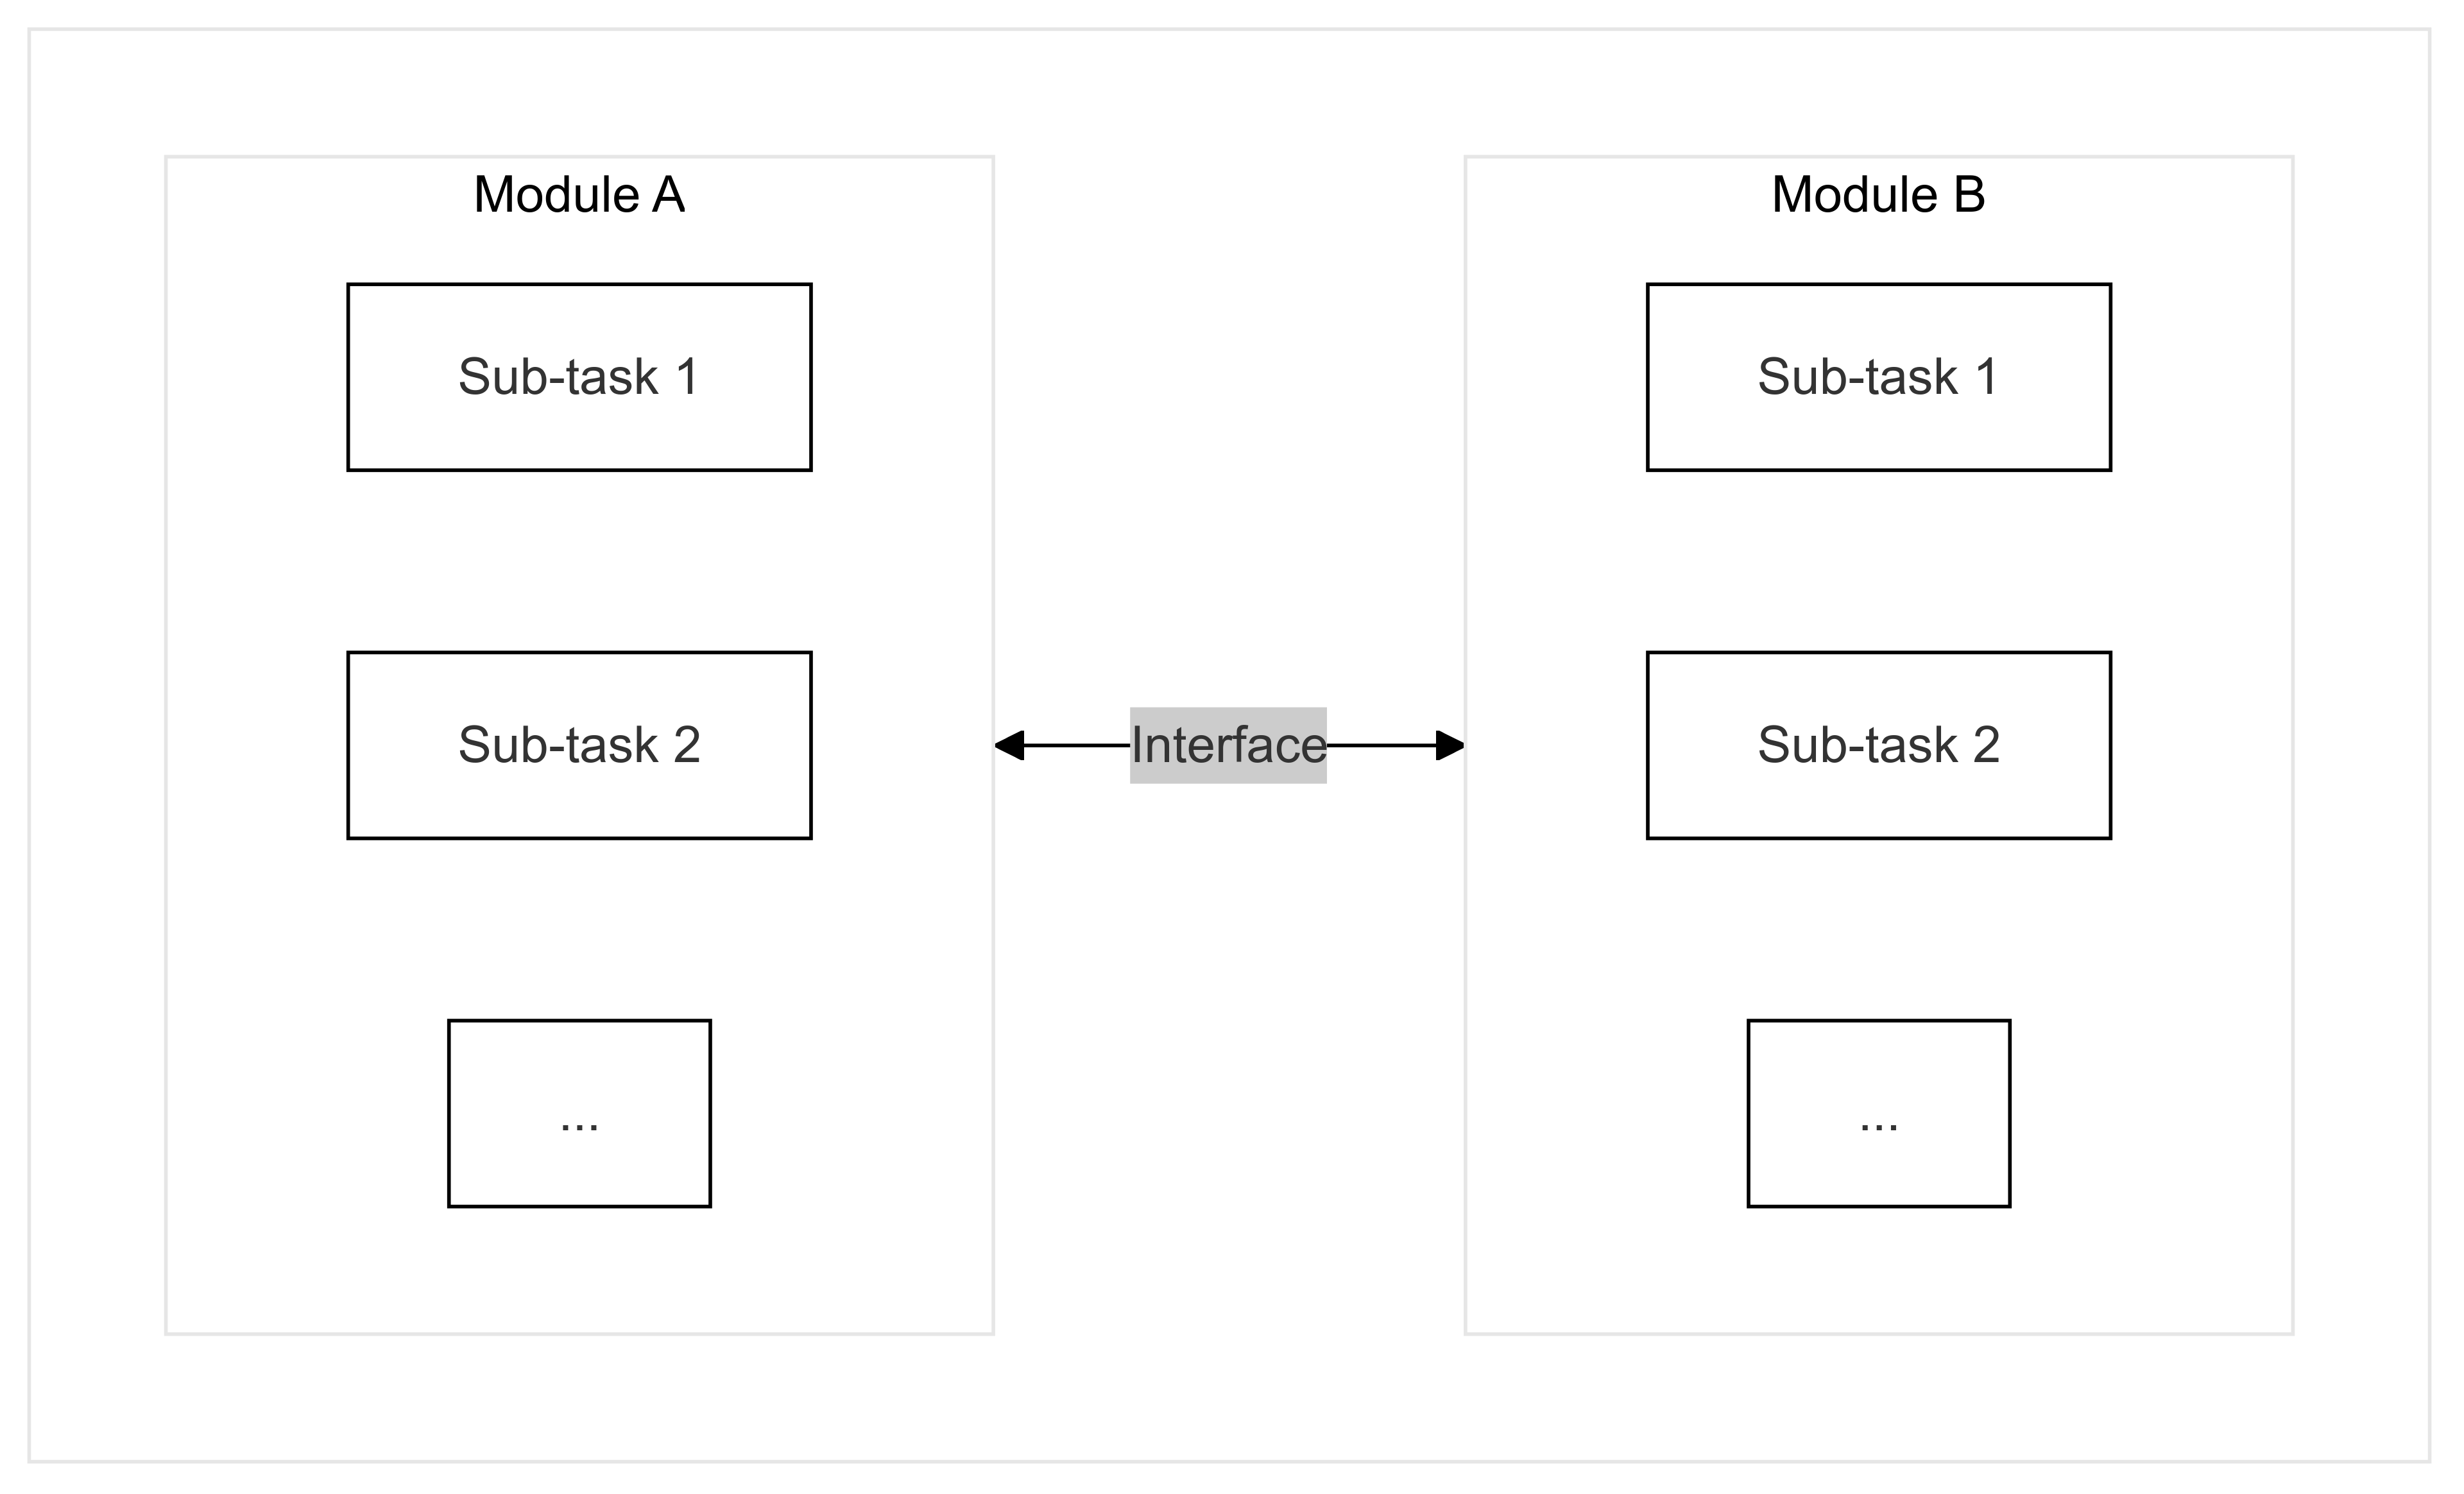
\includegraphics[width=0.7\textwidth]{modularity/horizontal.png}
%     \label{fig:mod_hor}
% \end{minipage}%
% \begin{minipage}{.6\textwidth}
%     \centering
%     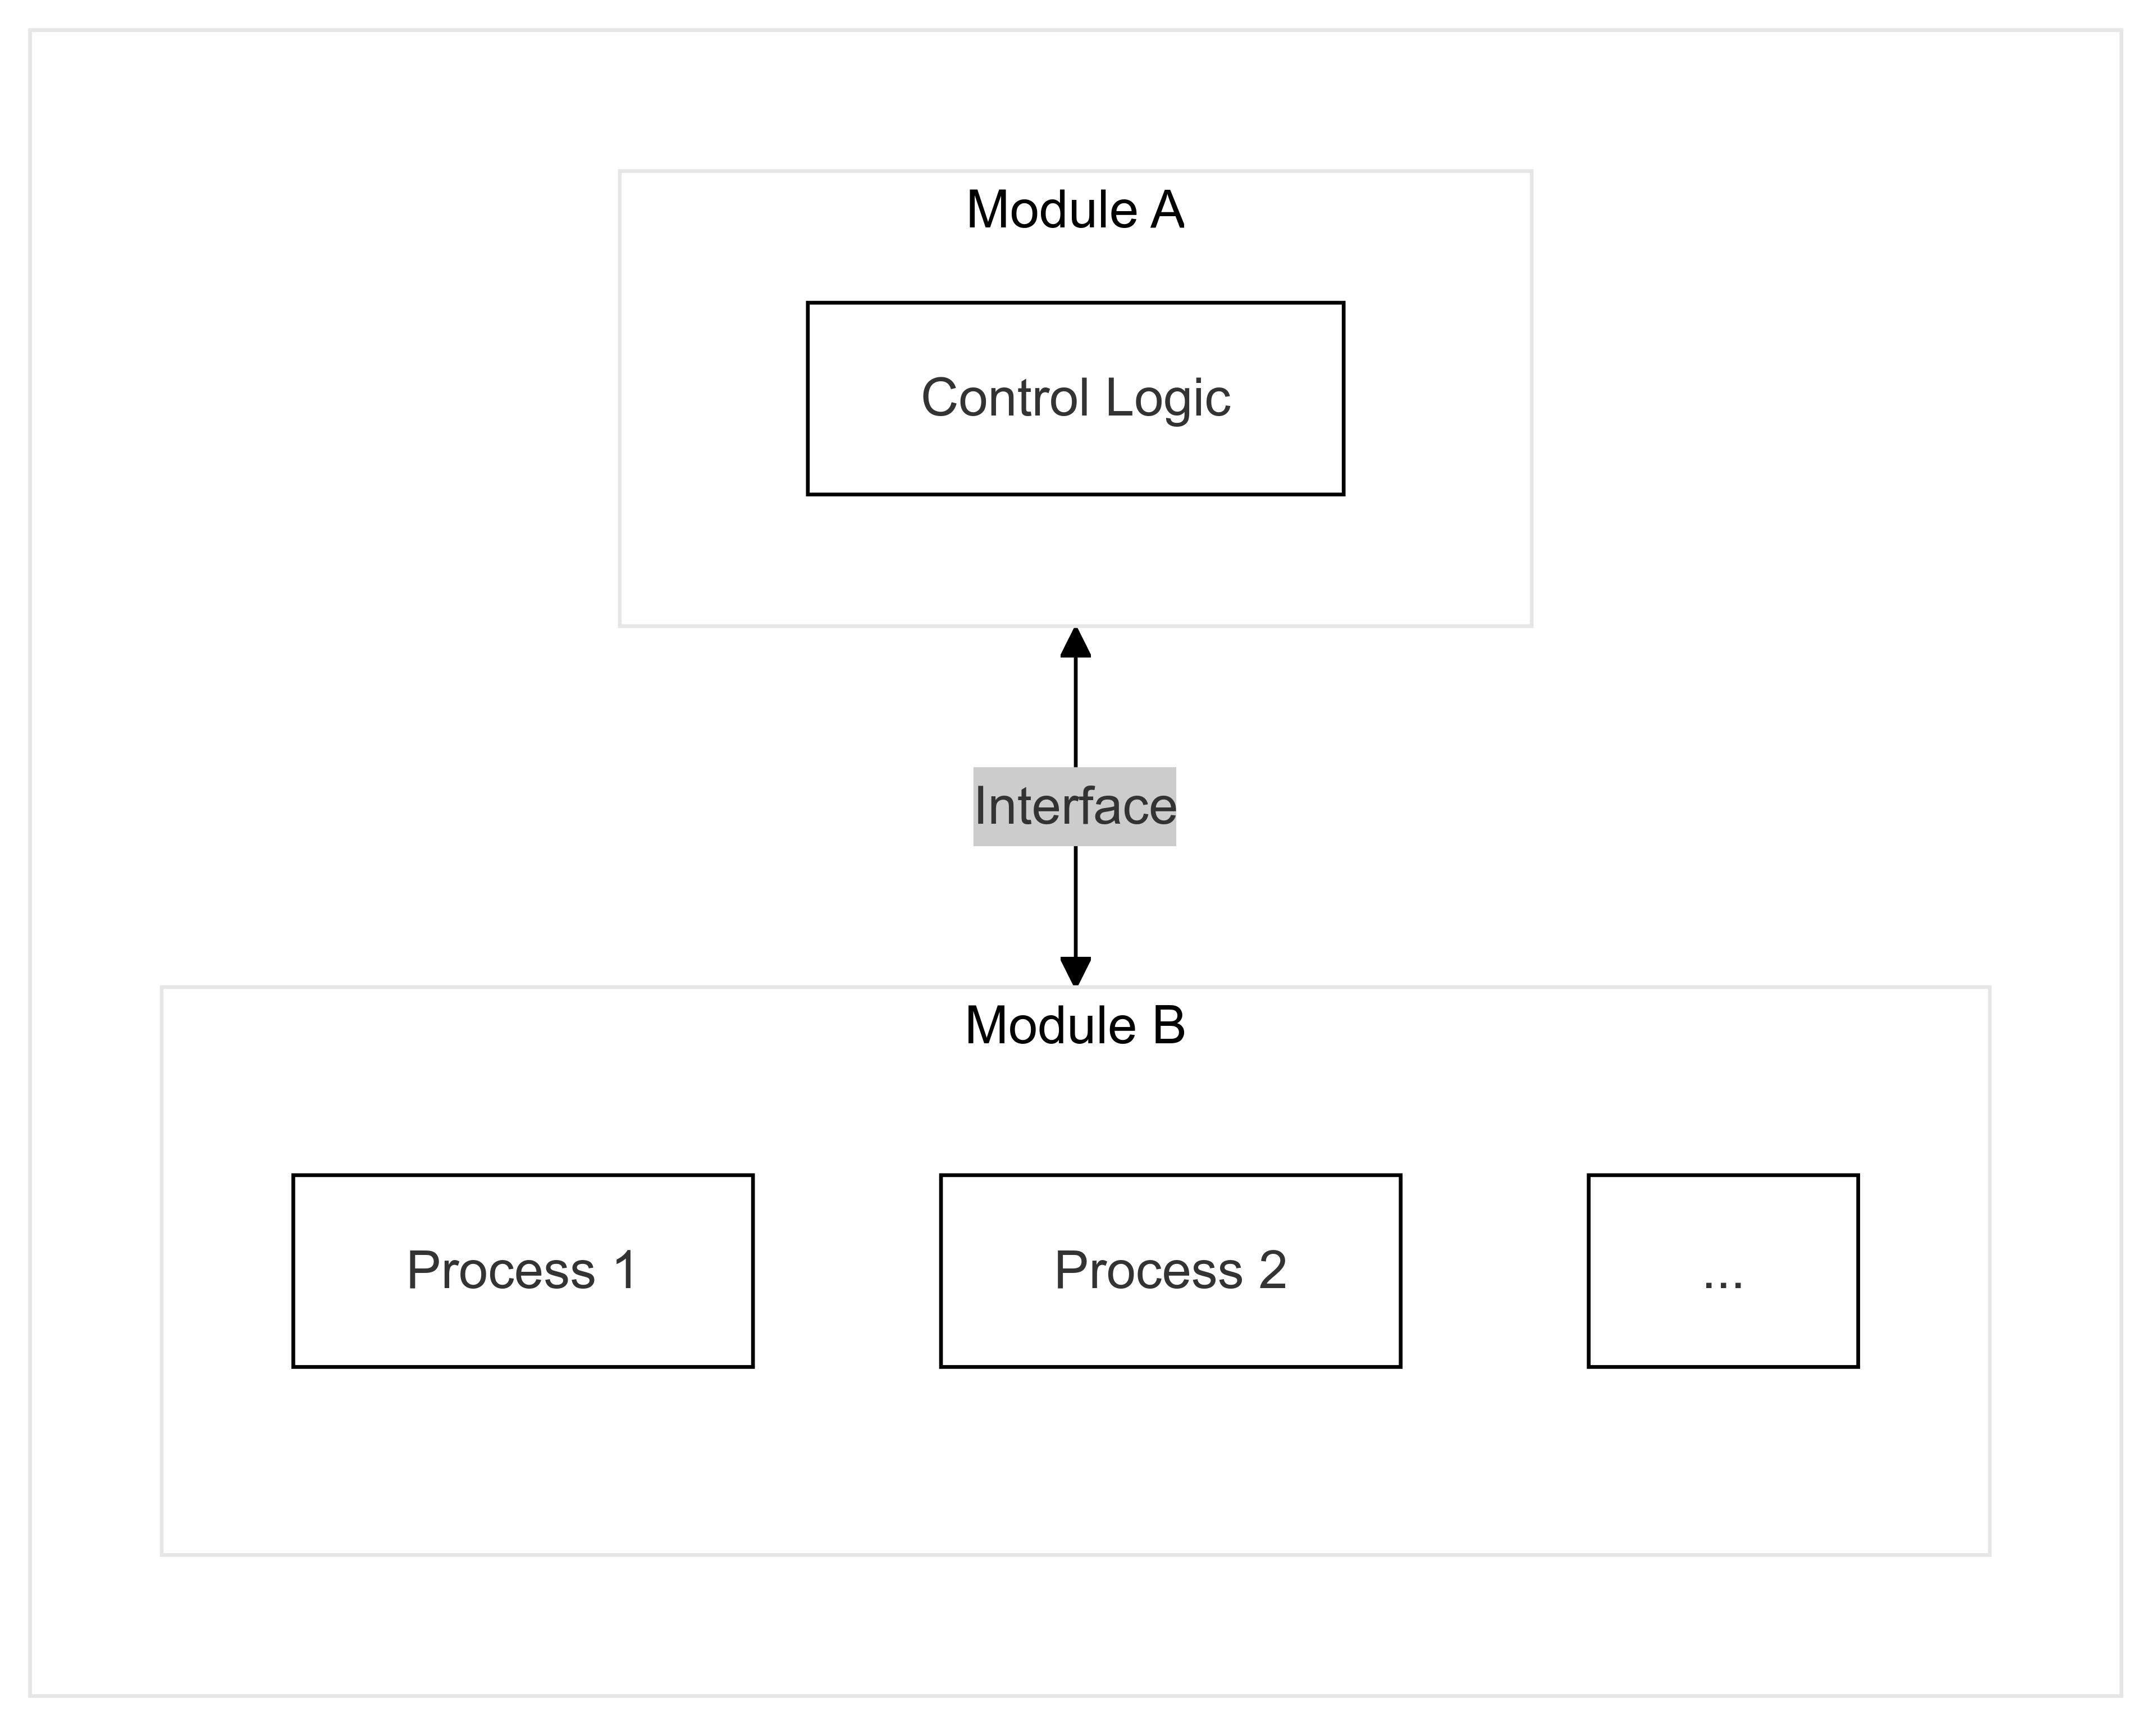
\includegraphics[width=0.7\textwidth]{modularity/vertical.png}
%     \label{fig:mod_ver}
% \end{minipage}
% \caption{Horizontal and vertical partitioning}
% \end{figure}

% \begin{figure}[hbt!]
%     \centering
%     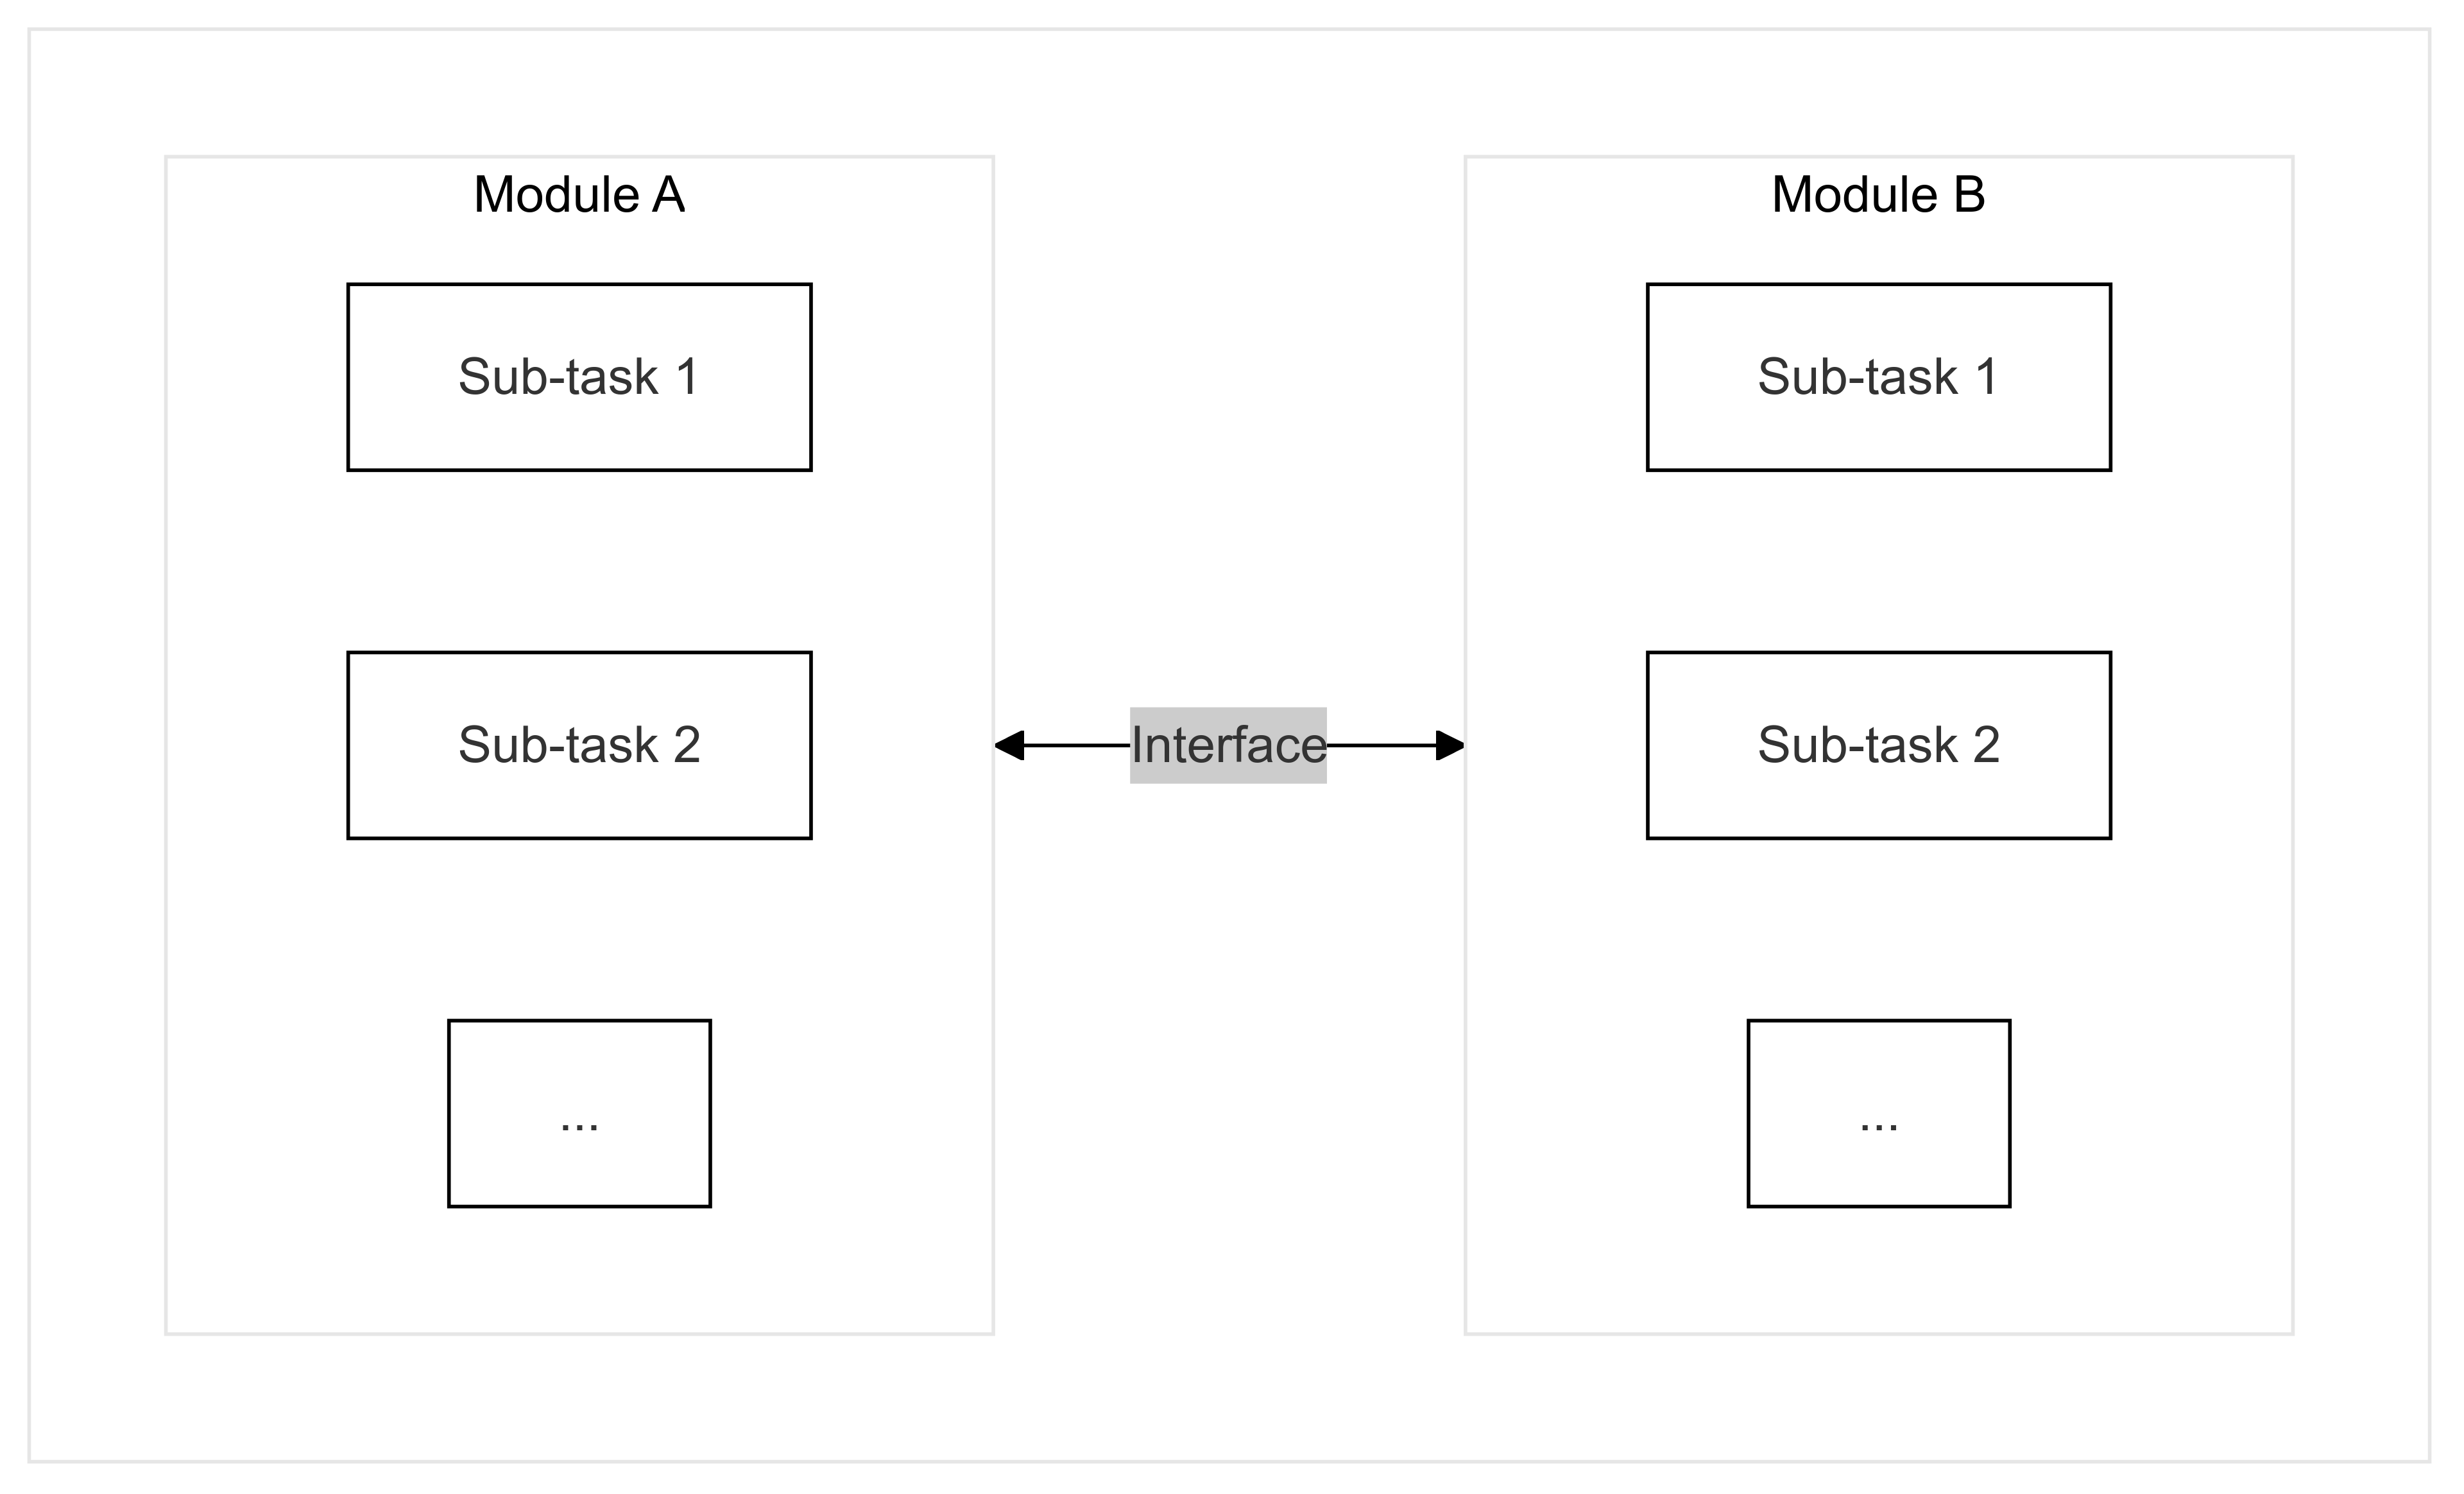
\includegraphics[width=0.7\textwidth]{modularity/horizontal.png}
%     \caption{Horizontal partitioning}
%     \label{fig:mod_hor}
% \end{figure}

% \begin{figure}[hbt!]
%     \centering
%     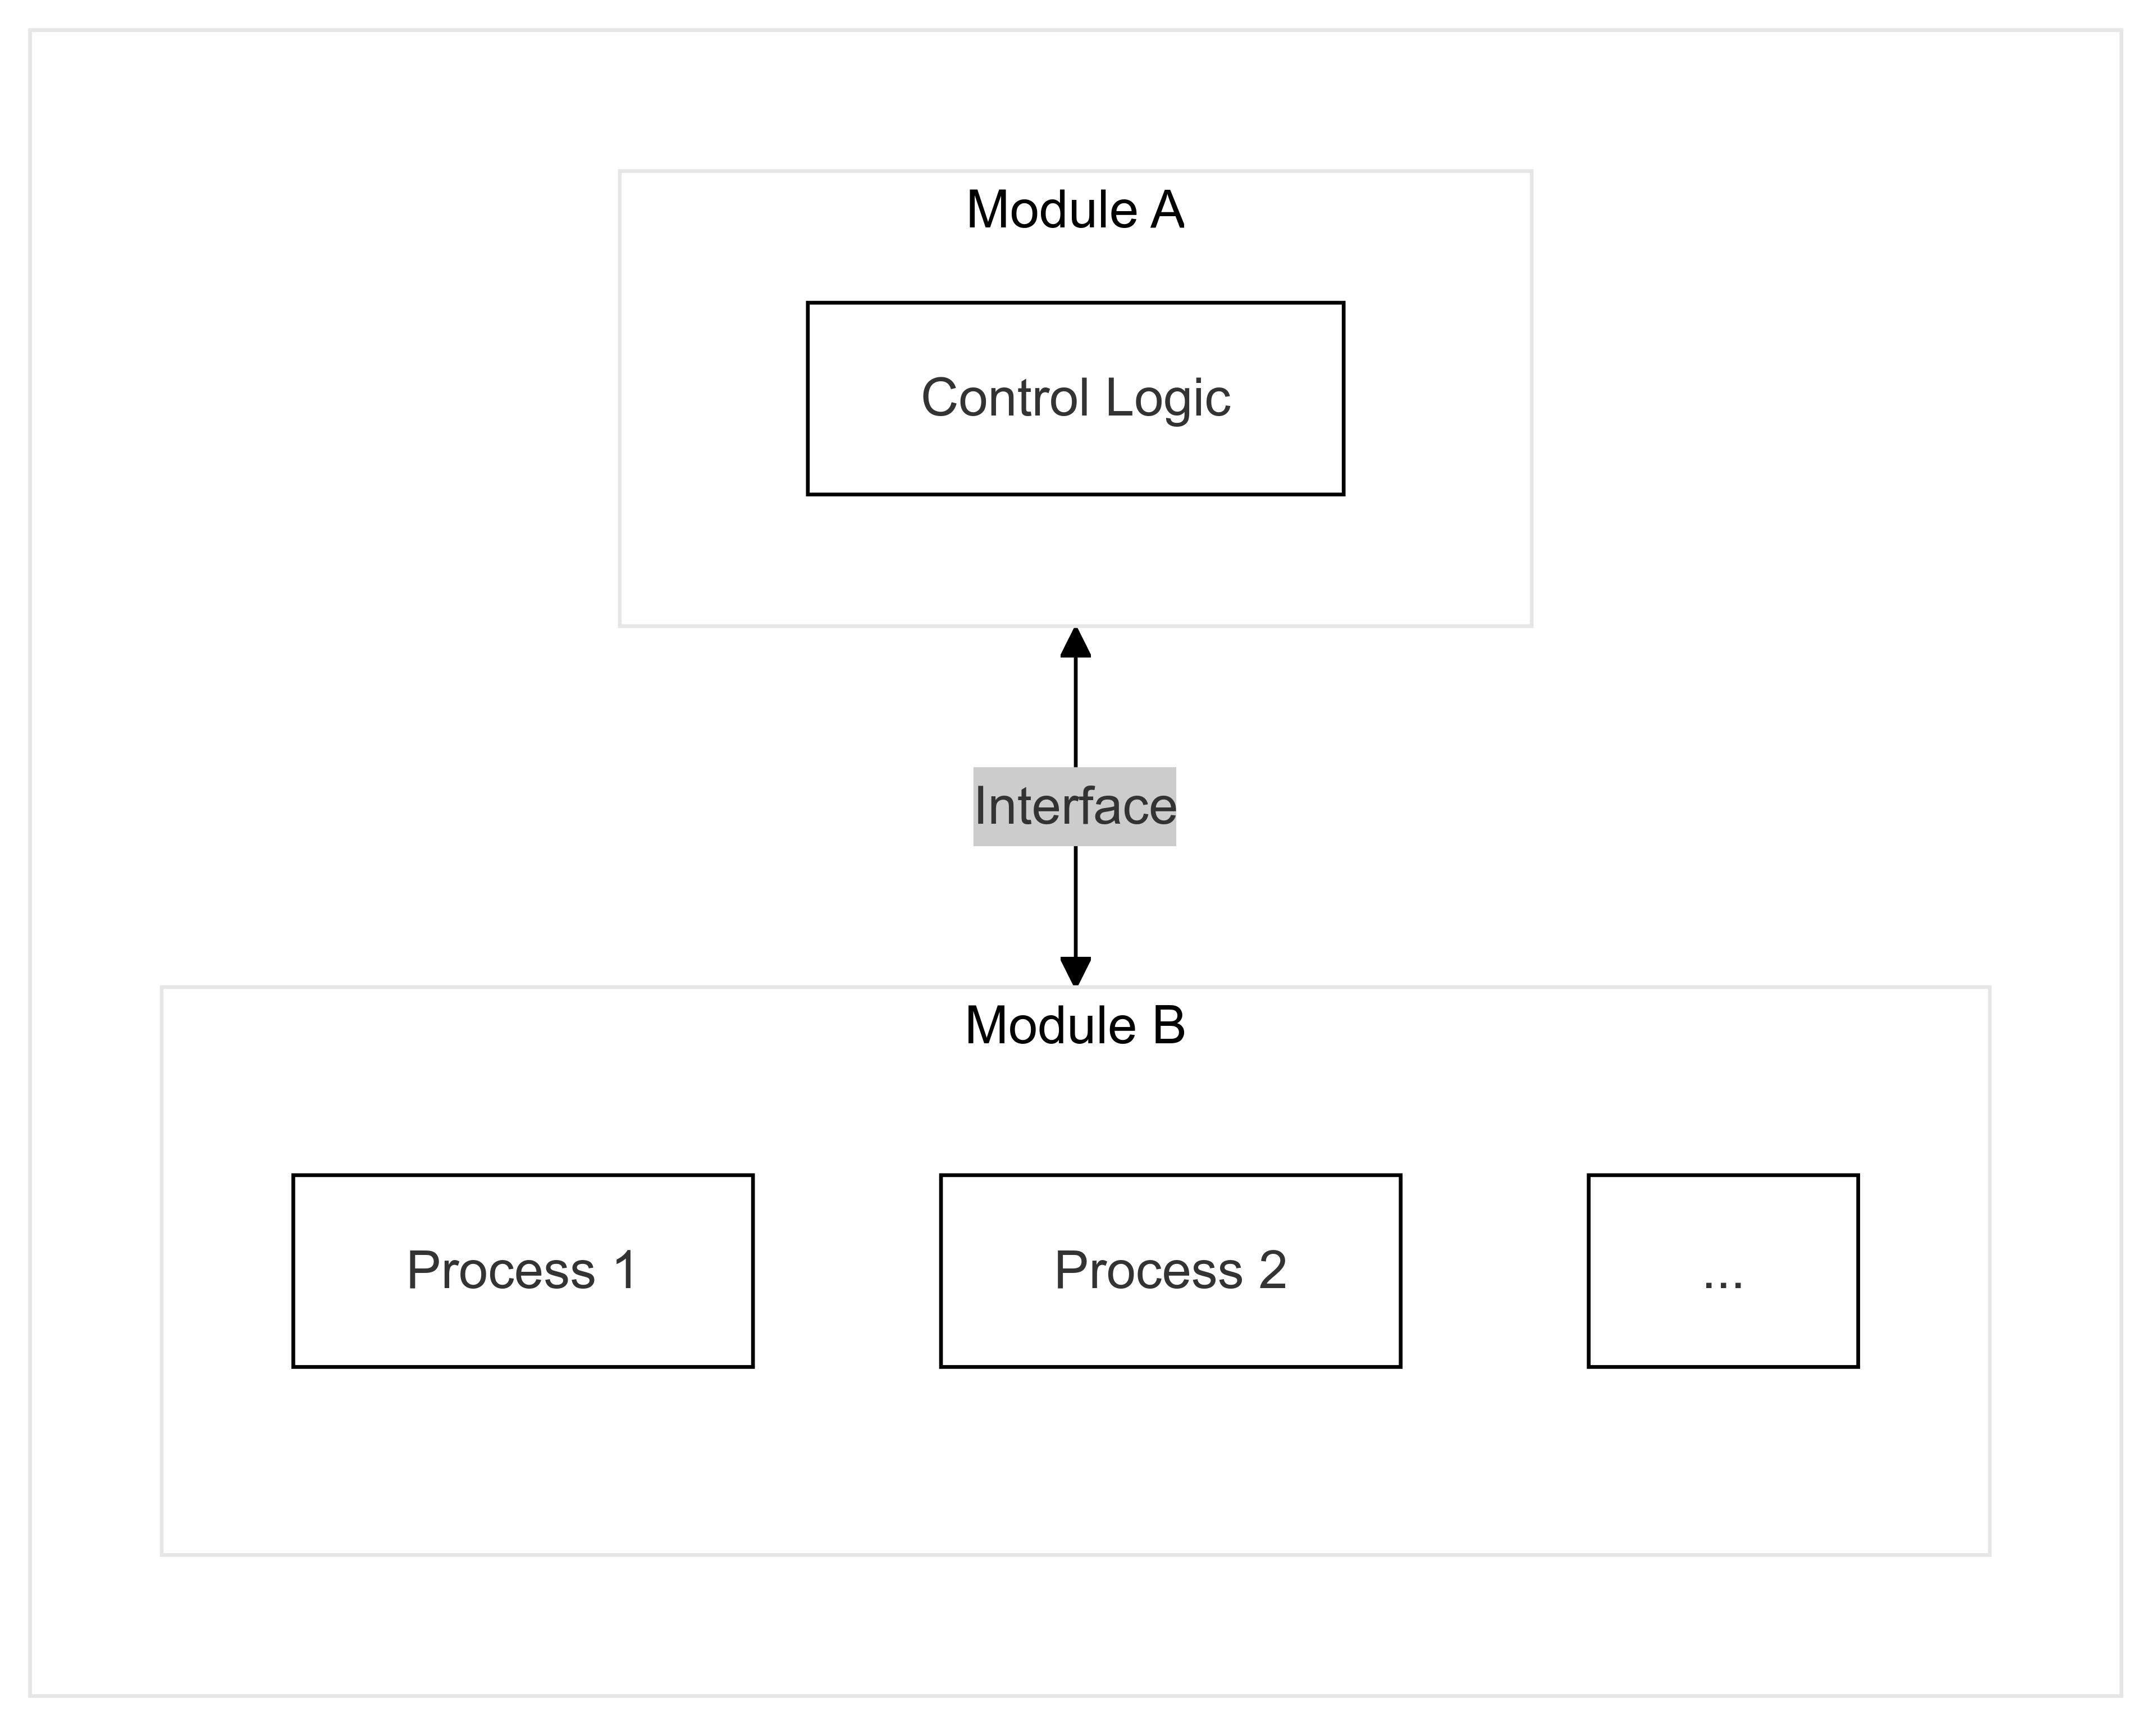
\includegraphics[width=0.7\textwidth]{modularity/vertical.png}
%     \caption{Vertical partitioning}
%     \label{fig:mod_ver}
% \end{figure}

Benefit of partitioning is the ability of software to isolate errors. Provided the software is correctly structured, an error occurring in a single module should not propagate to other modules. Meaning we can use modularity as a way to pinpoint the erroneous parts of software and attempt recovery. If recovery is not possible, the software should still be able to partially function, given that other parts of the software are not influenced by the fault. In most situations, partial functioning of a software is preferable to a complete shutdown.

\subsubsection{Error detection}

Fault-tolerant single-version application should meet two main criteria: self-protection and self-checking. Self-protection means that the application should be able to protect itself from external corruption by detecting errors in its input and output data as well as errors in its control flow. Self-checking means that the application component must be able to detect errors within itself and prevent propagation of these errors into other components \cite{nasa:sft}. These two traits combined can be together considered as the ability of "error detection".

Error detection covers a wide range of techniques used to locate errors and mitigate them. Some common approaches include:

a) checksums and \acrfullpl{ecc}, which embed additional metadata with the actual data in order to verify integrity and attempt to correct corrupted data. This approach allows for some degree of memory corruption mitigation but comes at the cost of memory overhead and additional processing per data-chunk which uses checksum or \acrshortpl{ecc}.

b) assertion and runtime checks, which perform independent checks on the data during execution which ensures the data matches the expected outcomes at certain checkpoints.

c) watchdog timers, whose main purpose is to catch deadlock states by giving a task a certain amount of time to execute before aborting it.

Error detection is a crucial aspect of single-version application, since there is no alternate version to fall back upon.

\subsubsection{Fault recovery}

Fault recovery is a process of restoring the program to a functional state after an error has been detected. Fault recovery in single-version techniques mostly consists of a program rollback. This can be either a full restart, effectively rolling back the program to its initial state, or a more advanced technique such as checkpoint and restart.

Checkpoint and restart could be considered the basis of some of the more advanced fault tolerance techniques. Before the execution of a critical process a checkpoint is created, which captures some or all of the program state. At the end of the execution, an acceptance check is performed on the process output, if an error is detected rollback is initiated and the process is restarted.

\begin{figure}[hbt]
    \centering
    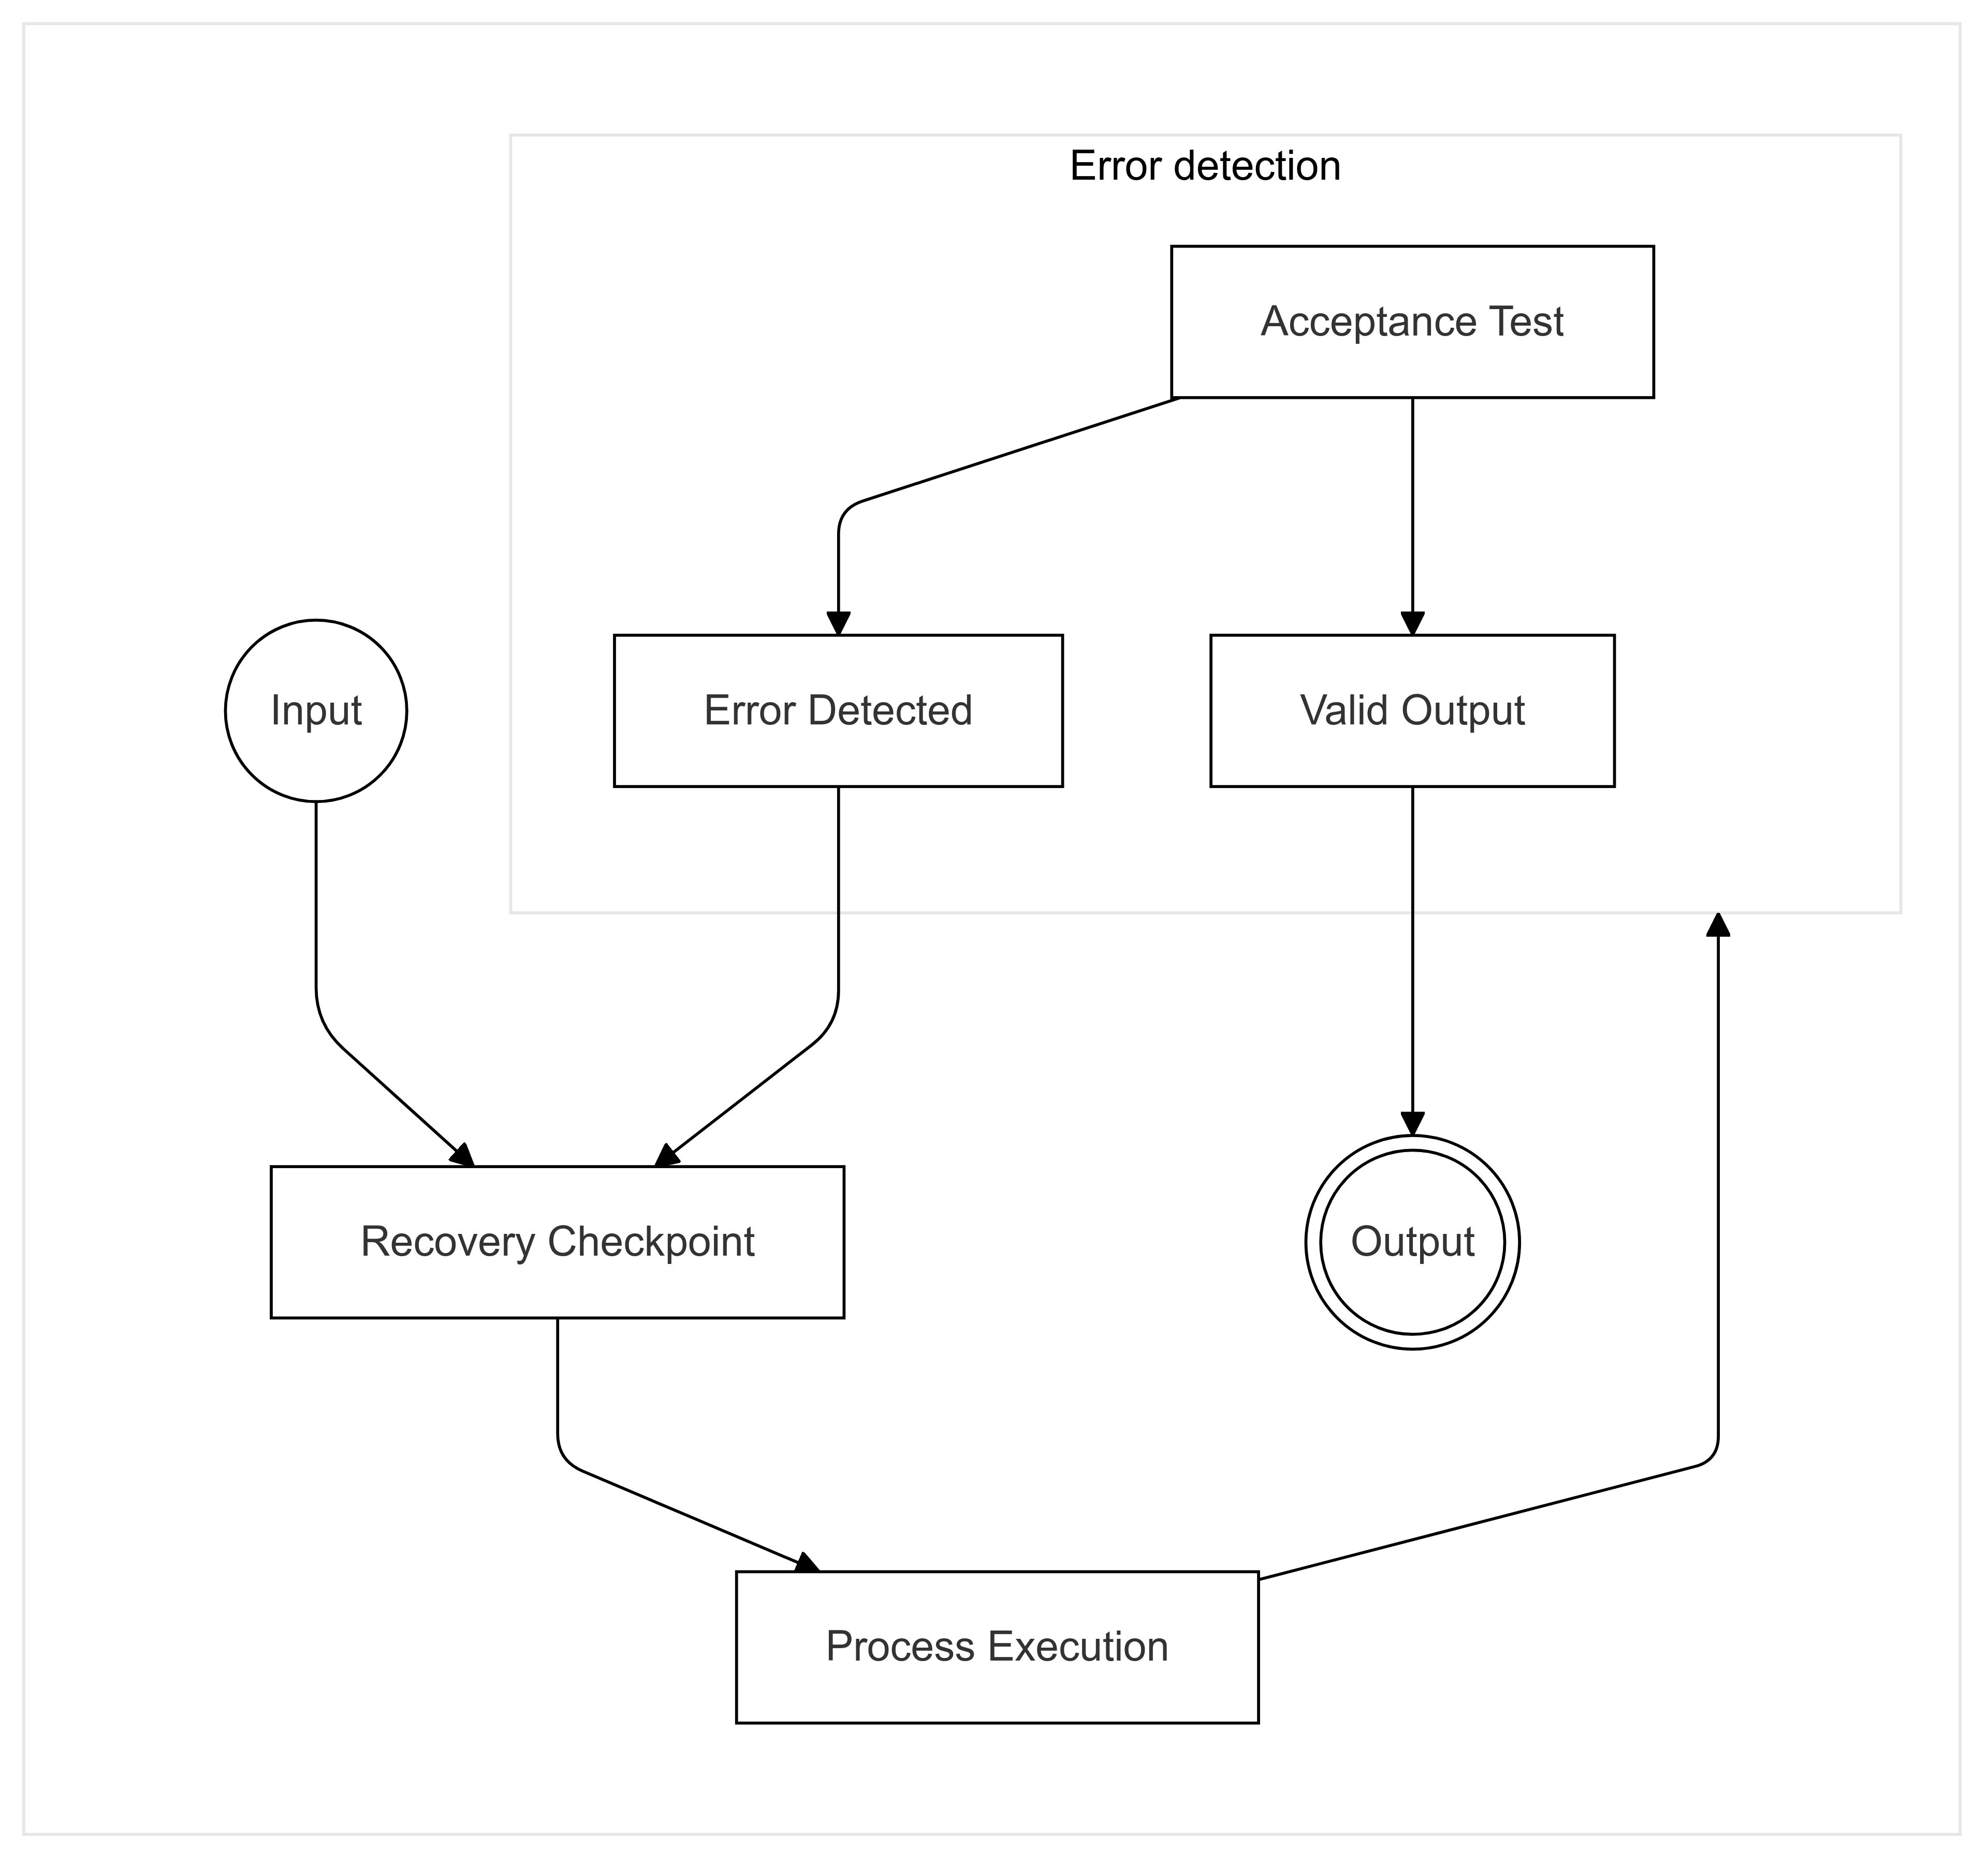
\includegraphics[width=0.8\textwidth]{diagrams/checkpoint/checkpoint.png}
    \caption{Checkpoint and restart}
    \label{fig:checkpoint}
\end{figure}

\subsubsection{Considerations for single-version techniques}

Single-version fault tolerance techniques are largely easier to develop when compared to the ones discussed in the following section. With this relative simplicity comes the drawback of not being well suited for some situations. While these techniques should work well for transient faults that are unlikely to reoccur, a single version fault-tolerant system will fail when attempting to deal with persistent faults. Even if an error is successfully detected, single version techniques provide no clear way of dealing with errors that stem from, or are heavily influenced by the design of the system. As an example, if the memory region containing a critical function has been permanently damaged, it matters not how many times we attempt to rerun the function, it will always cause an error. For this reason, single version techniques should be reserved for parts of software which are not mission critical.

In order to effectively deal with solid faults, we need to consider multi-version techniques covered in the following section. A lot of these techniques take inspiration from single version techniques, or even directly build on top of them.
\subsection{Multi-version} \label{multi}

Multi-version techniques build on the idea of multiple software versions which all meet the same specifications. The rational behind multiple version is that different components should fail differently \cite{nasa:sft}.
These versions are interchangeable in terms of their output, but each version executes differently from the rest, ensuring that no two version share the same resources.
Multiple versions of the same software are executed either in sequence or in parallel \cite{nasa:sft}, each utilizing different error detection and recovery methods, to have the highest probability of completing the task successfully.

\subsubsection{Recovery blocks}

Recovery blocks \cite{lyu:sft} is a simple form of multi-version programming, expanding upon the idea of "checkpoint and restart". Unlike its single version counterpart, however, recovery blocks does not re-execute the same code again, but instead chooses a different version to try next.

A key advantage of the recovery blocks technique is that, in most cases, the primary version will be the only one to execute \cite{lyu:sft}, allowing alternate versions to prioritize redundancy and safety over performance. This enables the design of backup versions with gradually reduced performance requirements, ensuring robust fallback options without excessive resource consumption.

% \begin{figure}[hbt!]
%     \centering
%     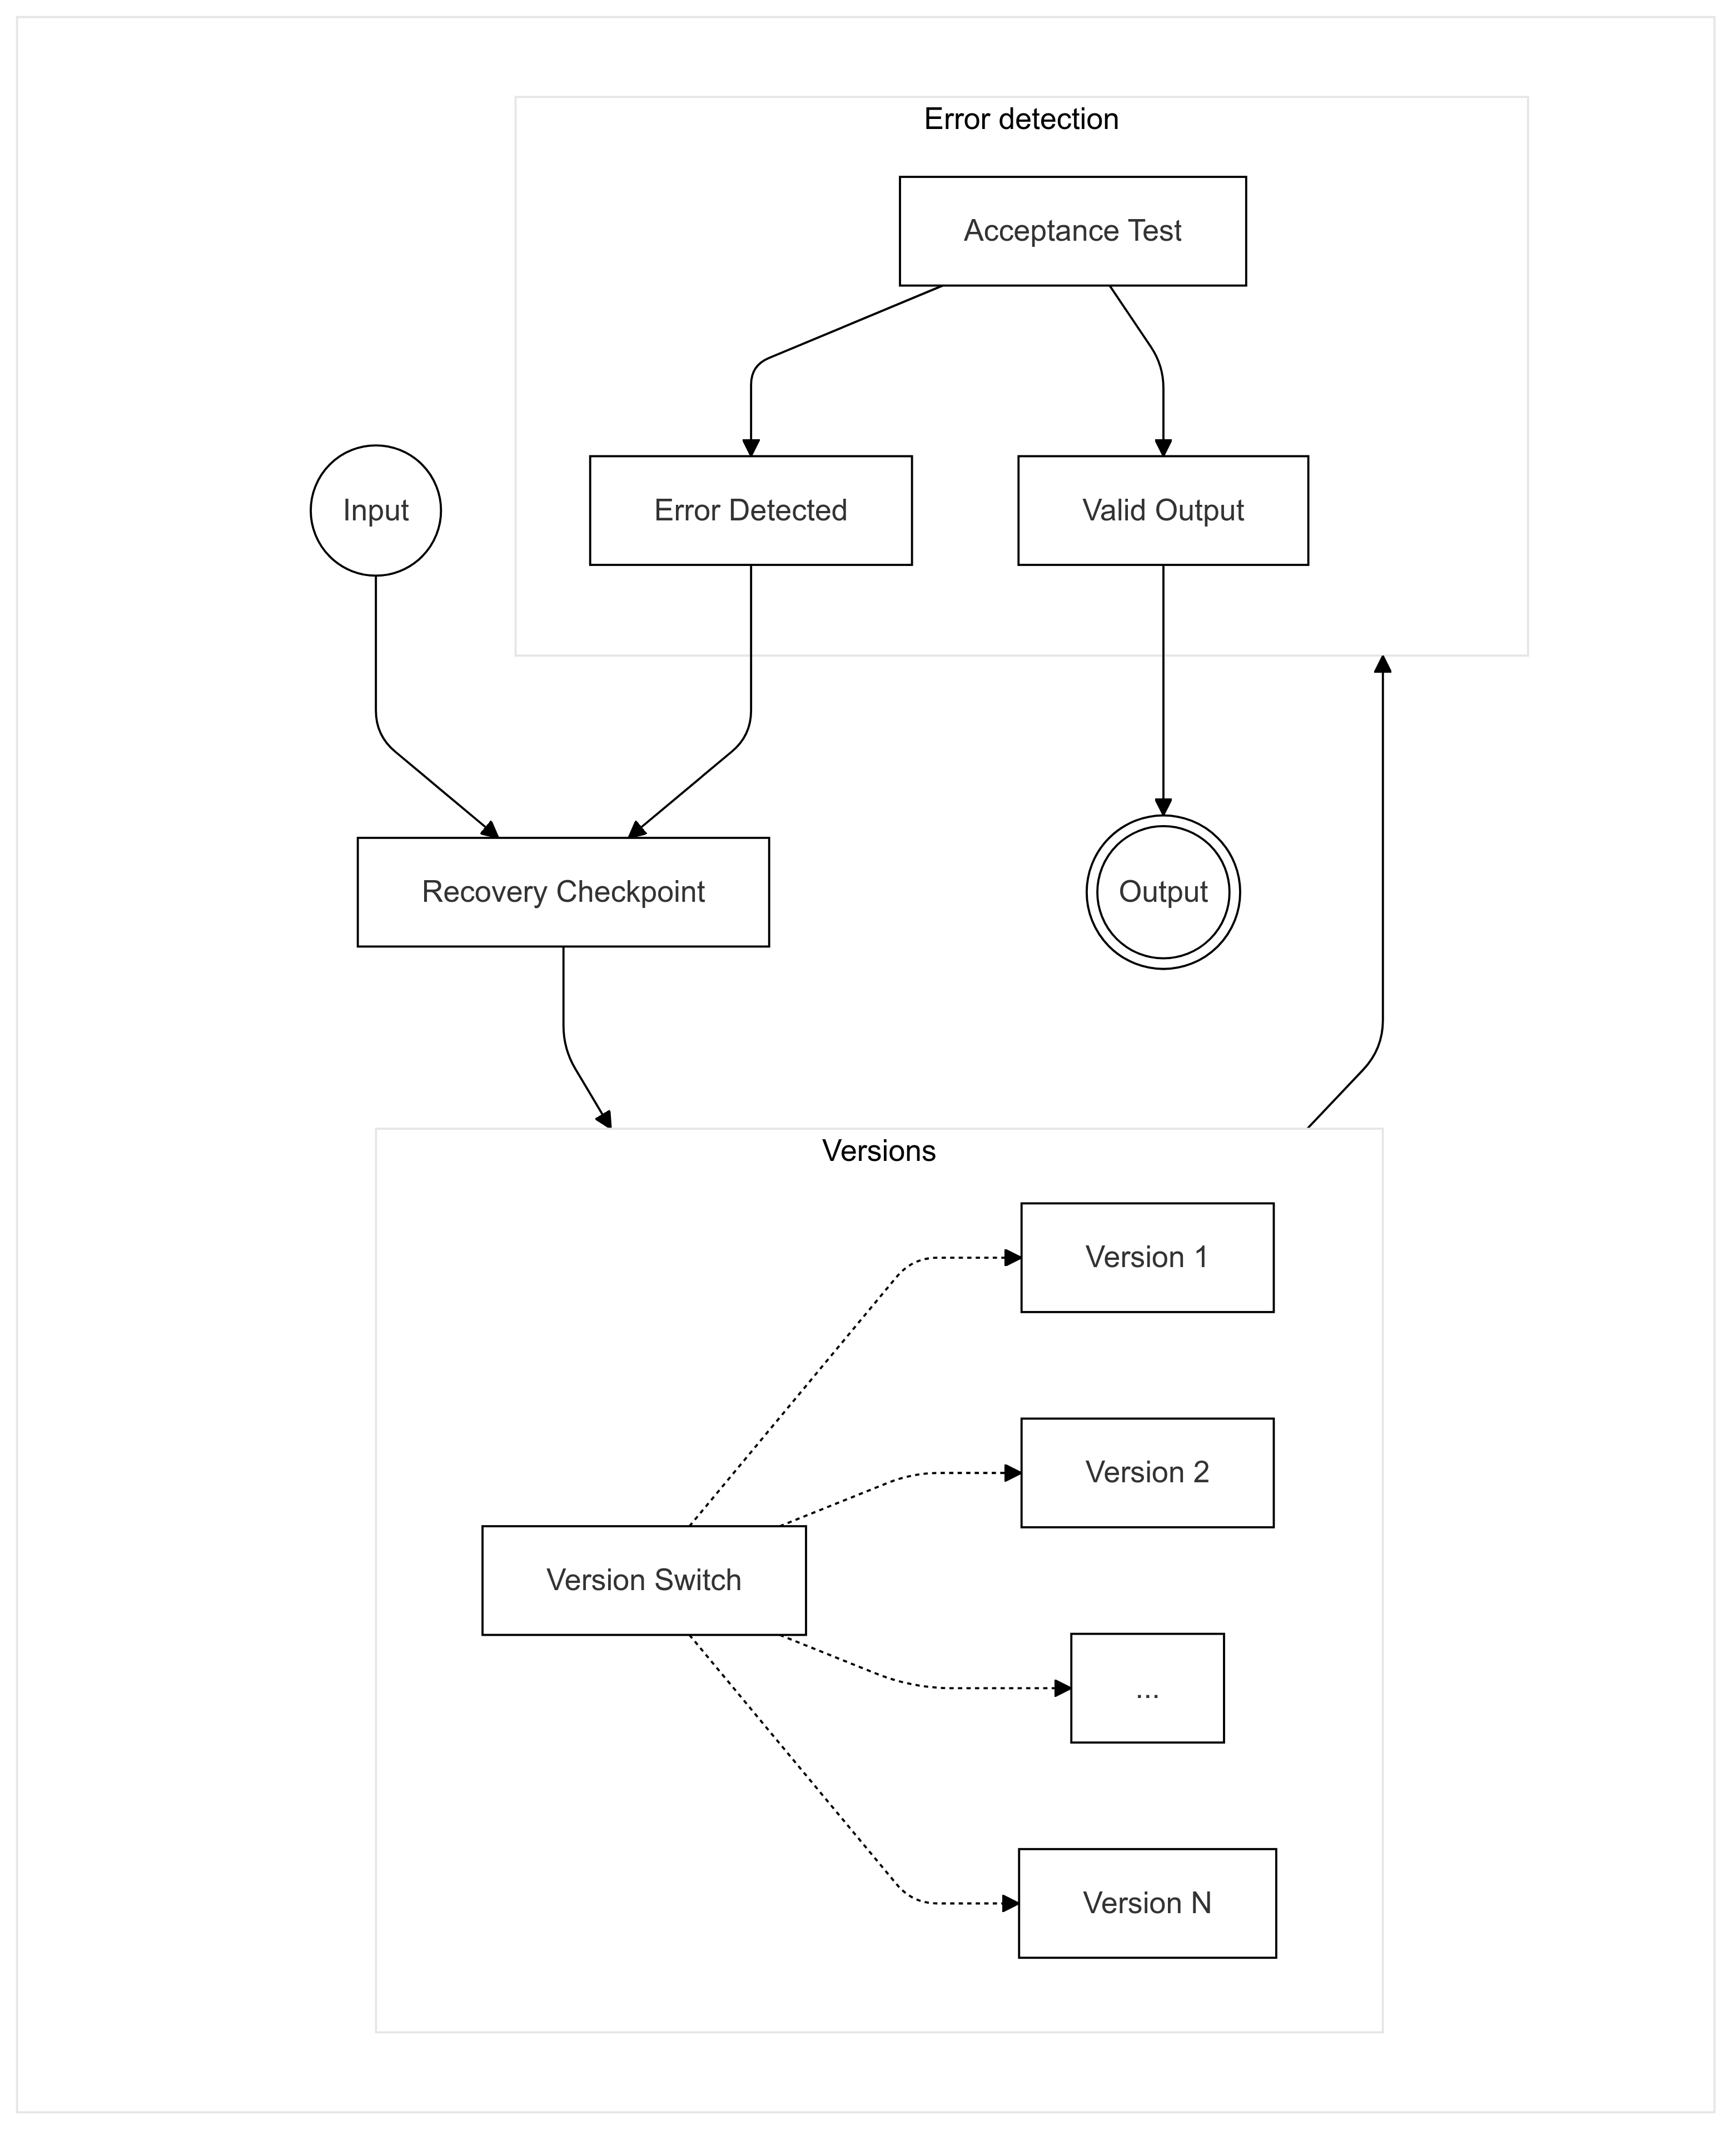
\includegraphics[width=0.9\textwidth]{recovery_blocks/recovery_blocks_01.png}
%     \caption{Recovery Blocks}
%     \label{fig:rec_blo}
% \end{figure}

% \break

In some situations, the alternate versions do not necessarily have to produce a correct result, but a result that satisfies the acceptance check \cite{lyu:sft}. Alternate version can gradually degrade the service in order to accomplish the bare minimum requirements.

The overall success of the recovery block scheme rests to a great extent on the effectiveness of the error detection mechanisms used — especially (but not solely) the acceptance test. The acceptance test must be simple otherwise there will be a significant chance that it will itself contain faults, and so fail to detect some errors, and/or falsely identify some conditions as being erroneous. Moreover, the test will introduce a run-time overhead which could be unacceptable if it is very complex. The development of simple, effective acceptance tests can thus be a difficult task, depending on the actual specification \cite{lyu:sft}.


\subsubsection{N-version programming}

\Acrfull{nvp} \cite{aa:nvp} extends the multi-version technique by running "N" independent versions in parallel or in sequence, hence “N-version” programming. In this approach, each version meeting the same specifications independently performs the task, and the final outcome is determined through a consensus mechanism that evaluates the results from all N executions.

This consensus is usually achieved through a voting algorithm, which aggregates the outputs from each version and selects the result agreed upon by the majority. Selection algorithms are an entire topic of its own covered well by \cite{Aljarbouh_2021}.

This voting approach to handling errors is sometimes referred to as \textbf{fault masking}, since we are not necessarily concerned with detecting an error, but rather getting an acceptable output even in the presence of a fault.

\begin{figure}[hbt!]
    \centering
    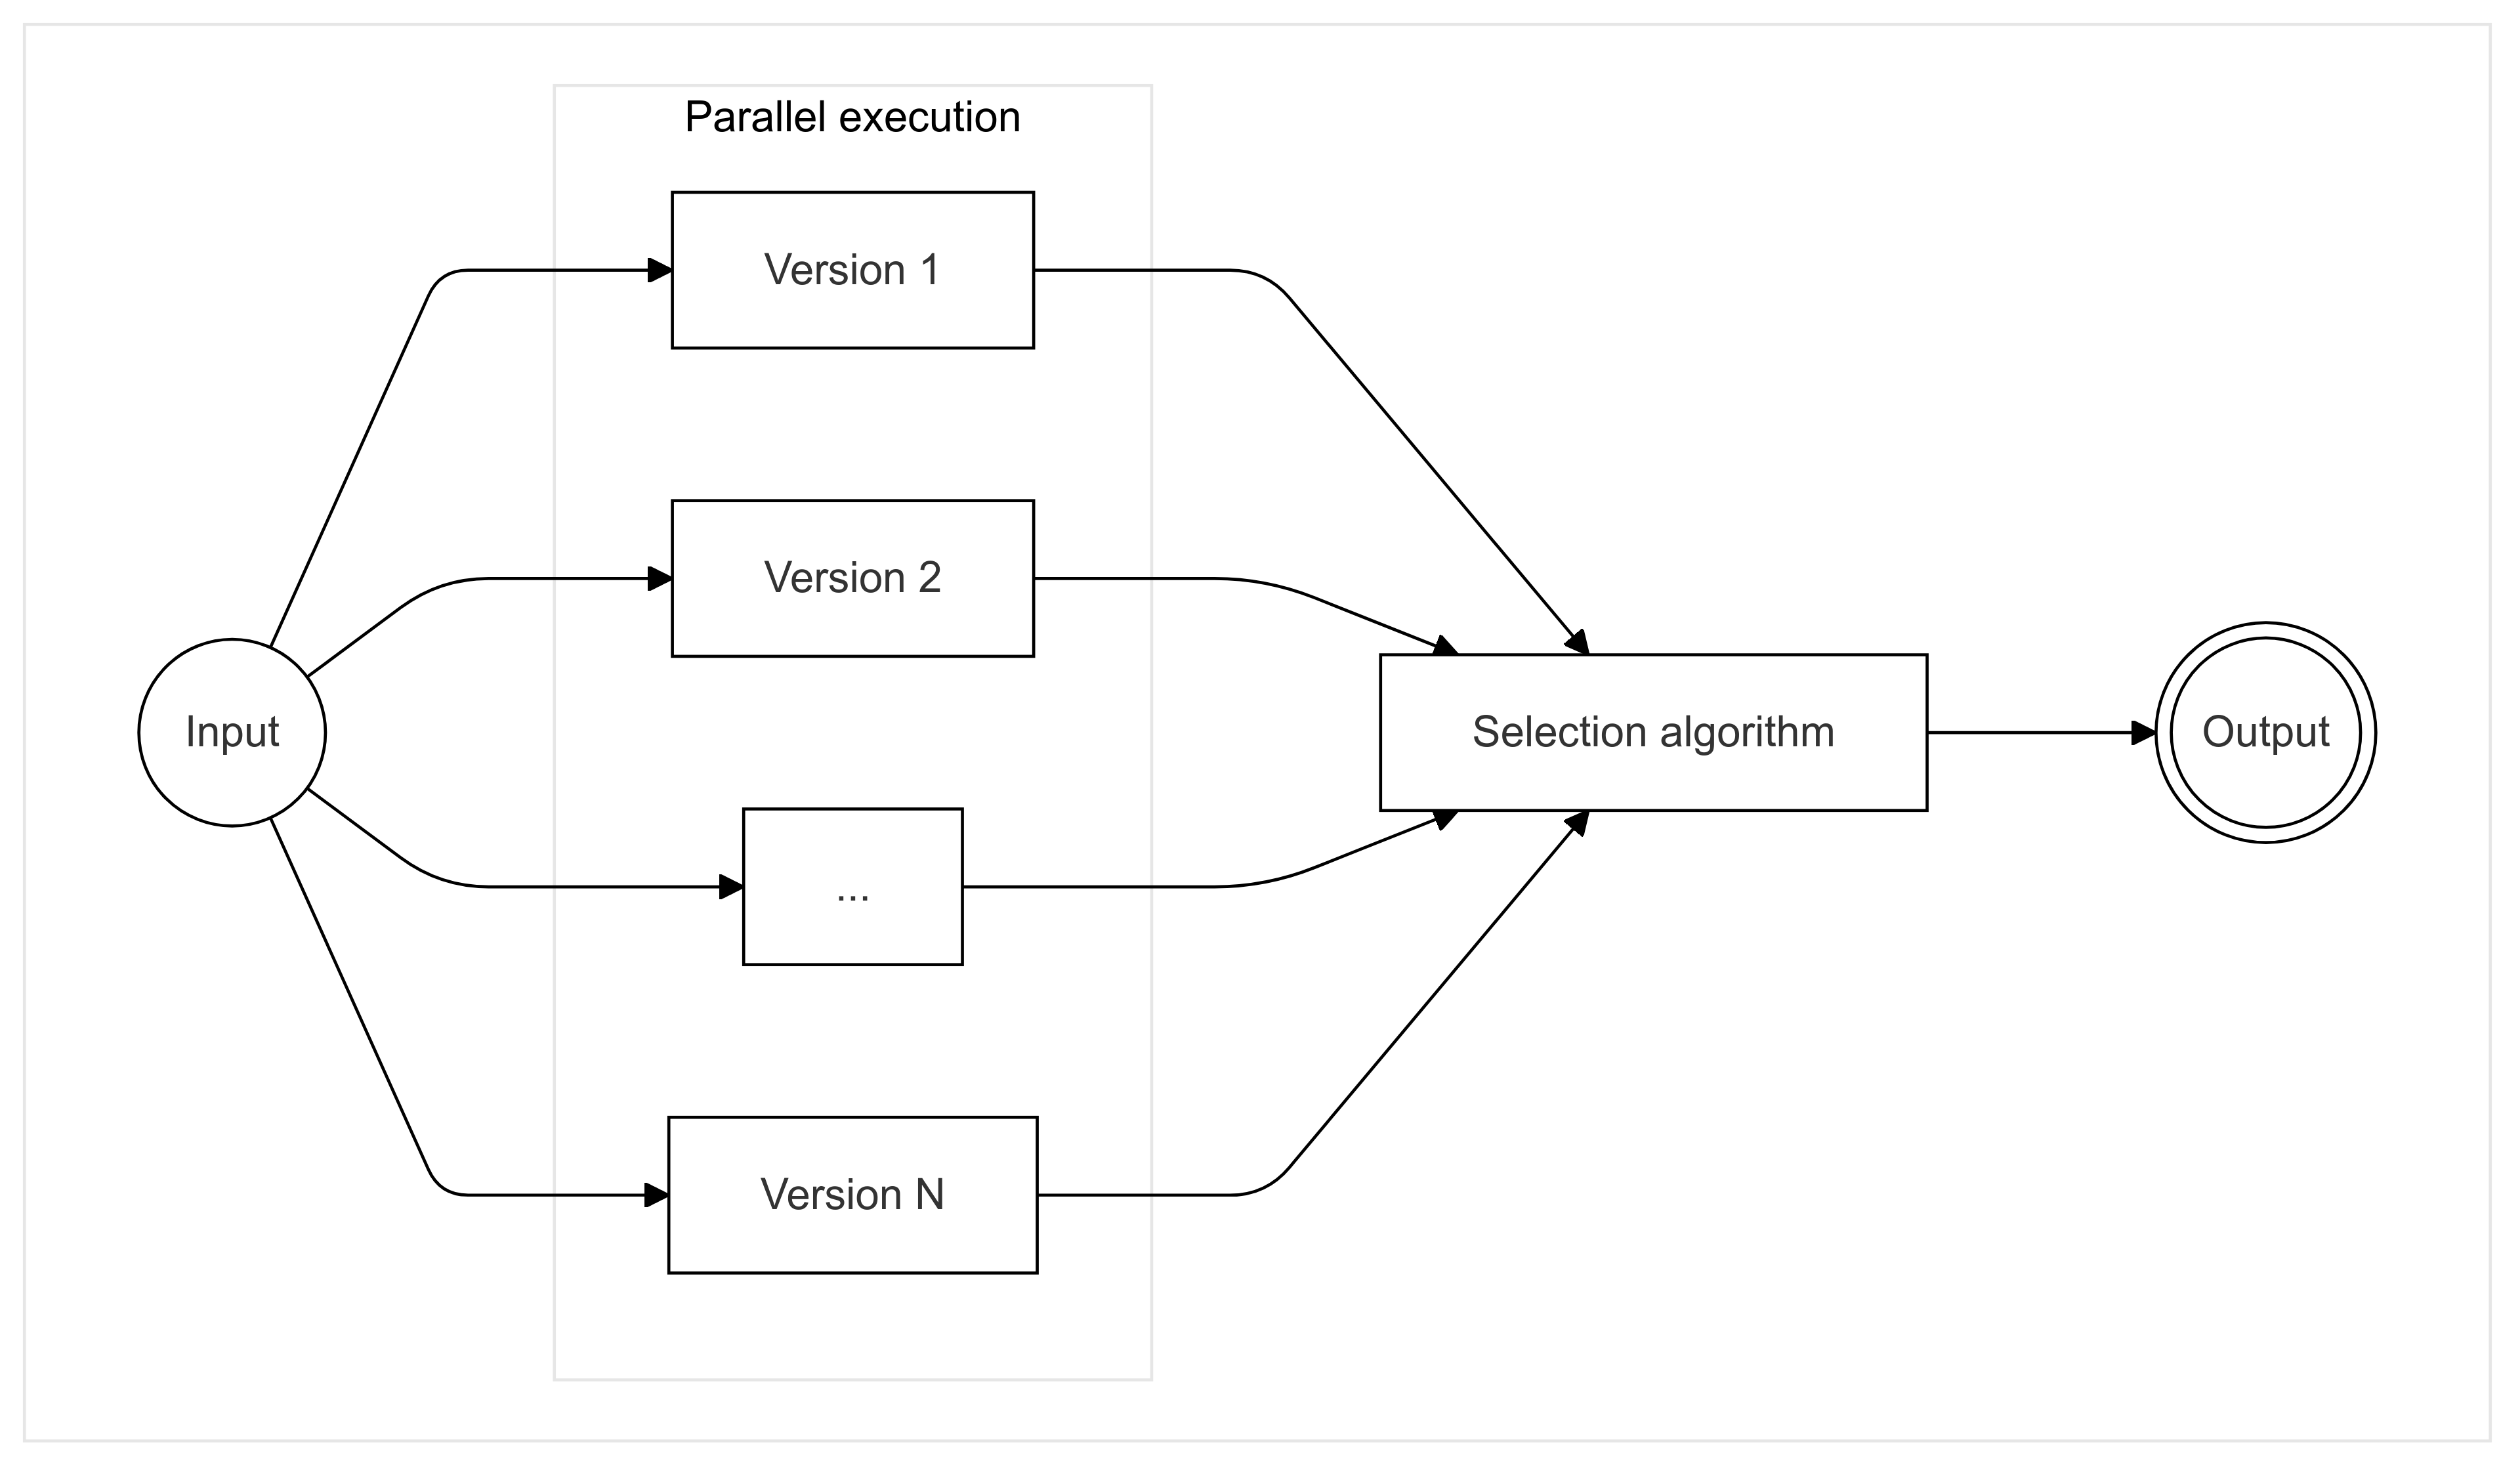
\includegraphics[width=0.9\textwidth]{n_version_prog/n_version_prog.png}
    \caption{N-Version Programming}
\end{figure}

The primary drawback of \acrshort{nvp} is its requirement to execute all of the versions before determining the final output. This can be highly resource intensive, especially for large or complex tasks, as it requires significant computational power and memory to run multiple versions simultaneously.

For systems with limited resources, such as embedded systems, this approach can be particularly inefficient. The need to allocate resources for each version can strain the system's capabilities, potentially reducing its overall performance and responsiveness. As a result, while \acrshort{nvp} enhances fault tolerance and reliability, it may not be suitable for applications where resource constraints are a priority or where processing efficiency is critical.

A consideration for \acrshort{nvp} is the possibility of an error not being a random event, but rather a function of the input variables \cite{5326}. Therefore, even multiple versions running in parallel could all fail and give erroneous results. This makes the selection algorithm a critical failure point which \acrshort{nvp} on its own does not address.

\subsubsection{N Self-checking programming}

\Acrfull{nscp} \cite{nscp} is an extension of the classic \acrshort{nvp}, where on top of executing multiple versions, each version also contains its own independent acceptance test or recovery block, before the results are passed to the selection logic. The selection logic then selects the "topmost" possible version that reports a correct output.

A version-specialized acceptance check is an interesting addition, as it provides the opportunity to take advantage of the version implementation details. We can specifically tailor the check to consider the inner workings of the version to detect errors and possibly even correct them before proceeding to the selection stage.

The drawback here is the increase in complexity over the more simple recovery blocks which uses a shared acceptance check, or the simple N-version approach which opts for masking instead. By creating more acceptance checks we are introducing more opportunities for errors to manifest, while also spend more resource on development.


\subsubsection{Considerations for multi-version programming}

The primary challenge associated with multi-version programming is the significant effort required to develop, test, and maintain several versions of software that perform the same function. This process can be resource-intensive, leading to increased costs, making it unfeasible for smaller projects or for teams with a limited budget.

To achieve effective multi-version programming, each version must be carefully designed to execute the same task while incorporating distinct failure mechanisms. Ensuring that no two versions fail in the exact same way is very difficult and in practice not always possible.

Research has been conducted into other methods that improve upon the aforementioned multi-version techniques, such as the "t/(n-1)-Variant programming" \cite{589928} - extension of \acrshort{nvp} which uses fewer comparisons as opposed to \acrshort{nvp} or \acrshort{nscp} and can tolerate up to \textit{t} faults. However, the findings do not conclusively prove that the sharp increase in complexity justifies the marginal benefits this improved technique provides.
\subsection{Data diversity}

Faults within the data are the second largest cause of errors \cite{nasa:stats}, with that in mind, it is sometimes not enough to execute different version of a software on the same data in order to get an acceptable output. Instead, \textit{data diversity} \cite{nasa:datadiversity} might be required to ensure correct execution. Data diversity is an orthogonal method to the previously mentioned design diversity methods. It can be used on its own, or in combination with other fault tolerance methods.

\subsubsection{Failure regions}

In many situations only very specific conditions will result in an error, we call these specific condition edge-cases. Even with thorough testing, there is no guarantee that all edge-cases will be caught during development, since the \textit{failure domain} (the set of input points that cause program failure \cite{dd:sft}) can be extremely small. We can take advantage of this, however, by using "reexpressed" input on a subsequent execution of a procedure, since even small adjustments of the input are likely to move it away from the failure domain. 
 
\subsubsection{Data reexpression}

Data reexpression is generation of logically equivalent data sets. Any mapping of a program's data that preserves the information content of the data is a valid reexpression algorithm \cite{nasa:datadiversity}. A simple approximate data reexpression algorithm for a floating-point quantity might alter its value by a small percentage. Similar concept can also be found in \textit{approximate computing} \cite{approxcomp}. The allowable percentage by which the data value could be altered would be determined by the application. In applications that process sensor data, for example, the accuracy of the data is often poor and deliberate small changes are unlikely to affect performance \cite{nasa:datadiversity}. 

% \begin{figure}[hbt]
%     \centering
%     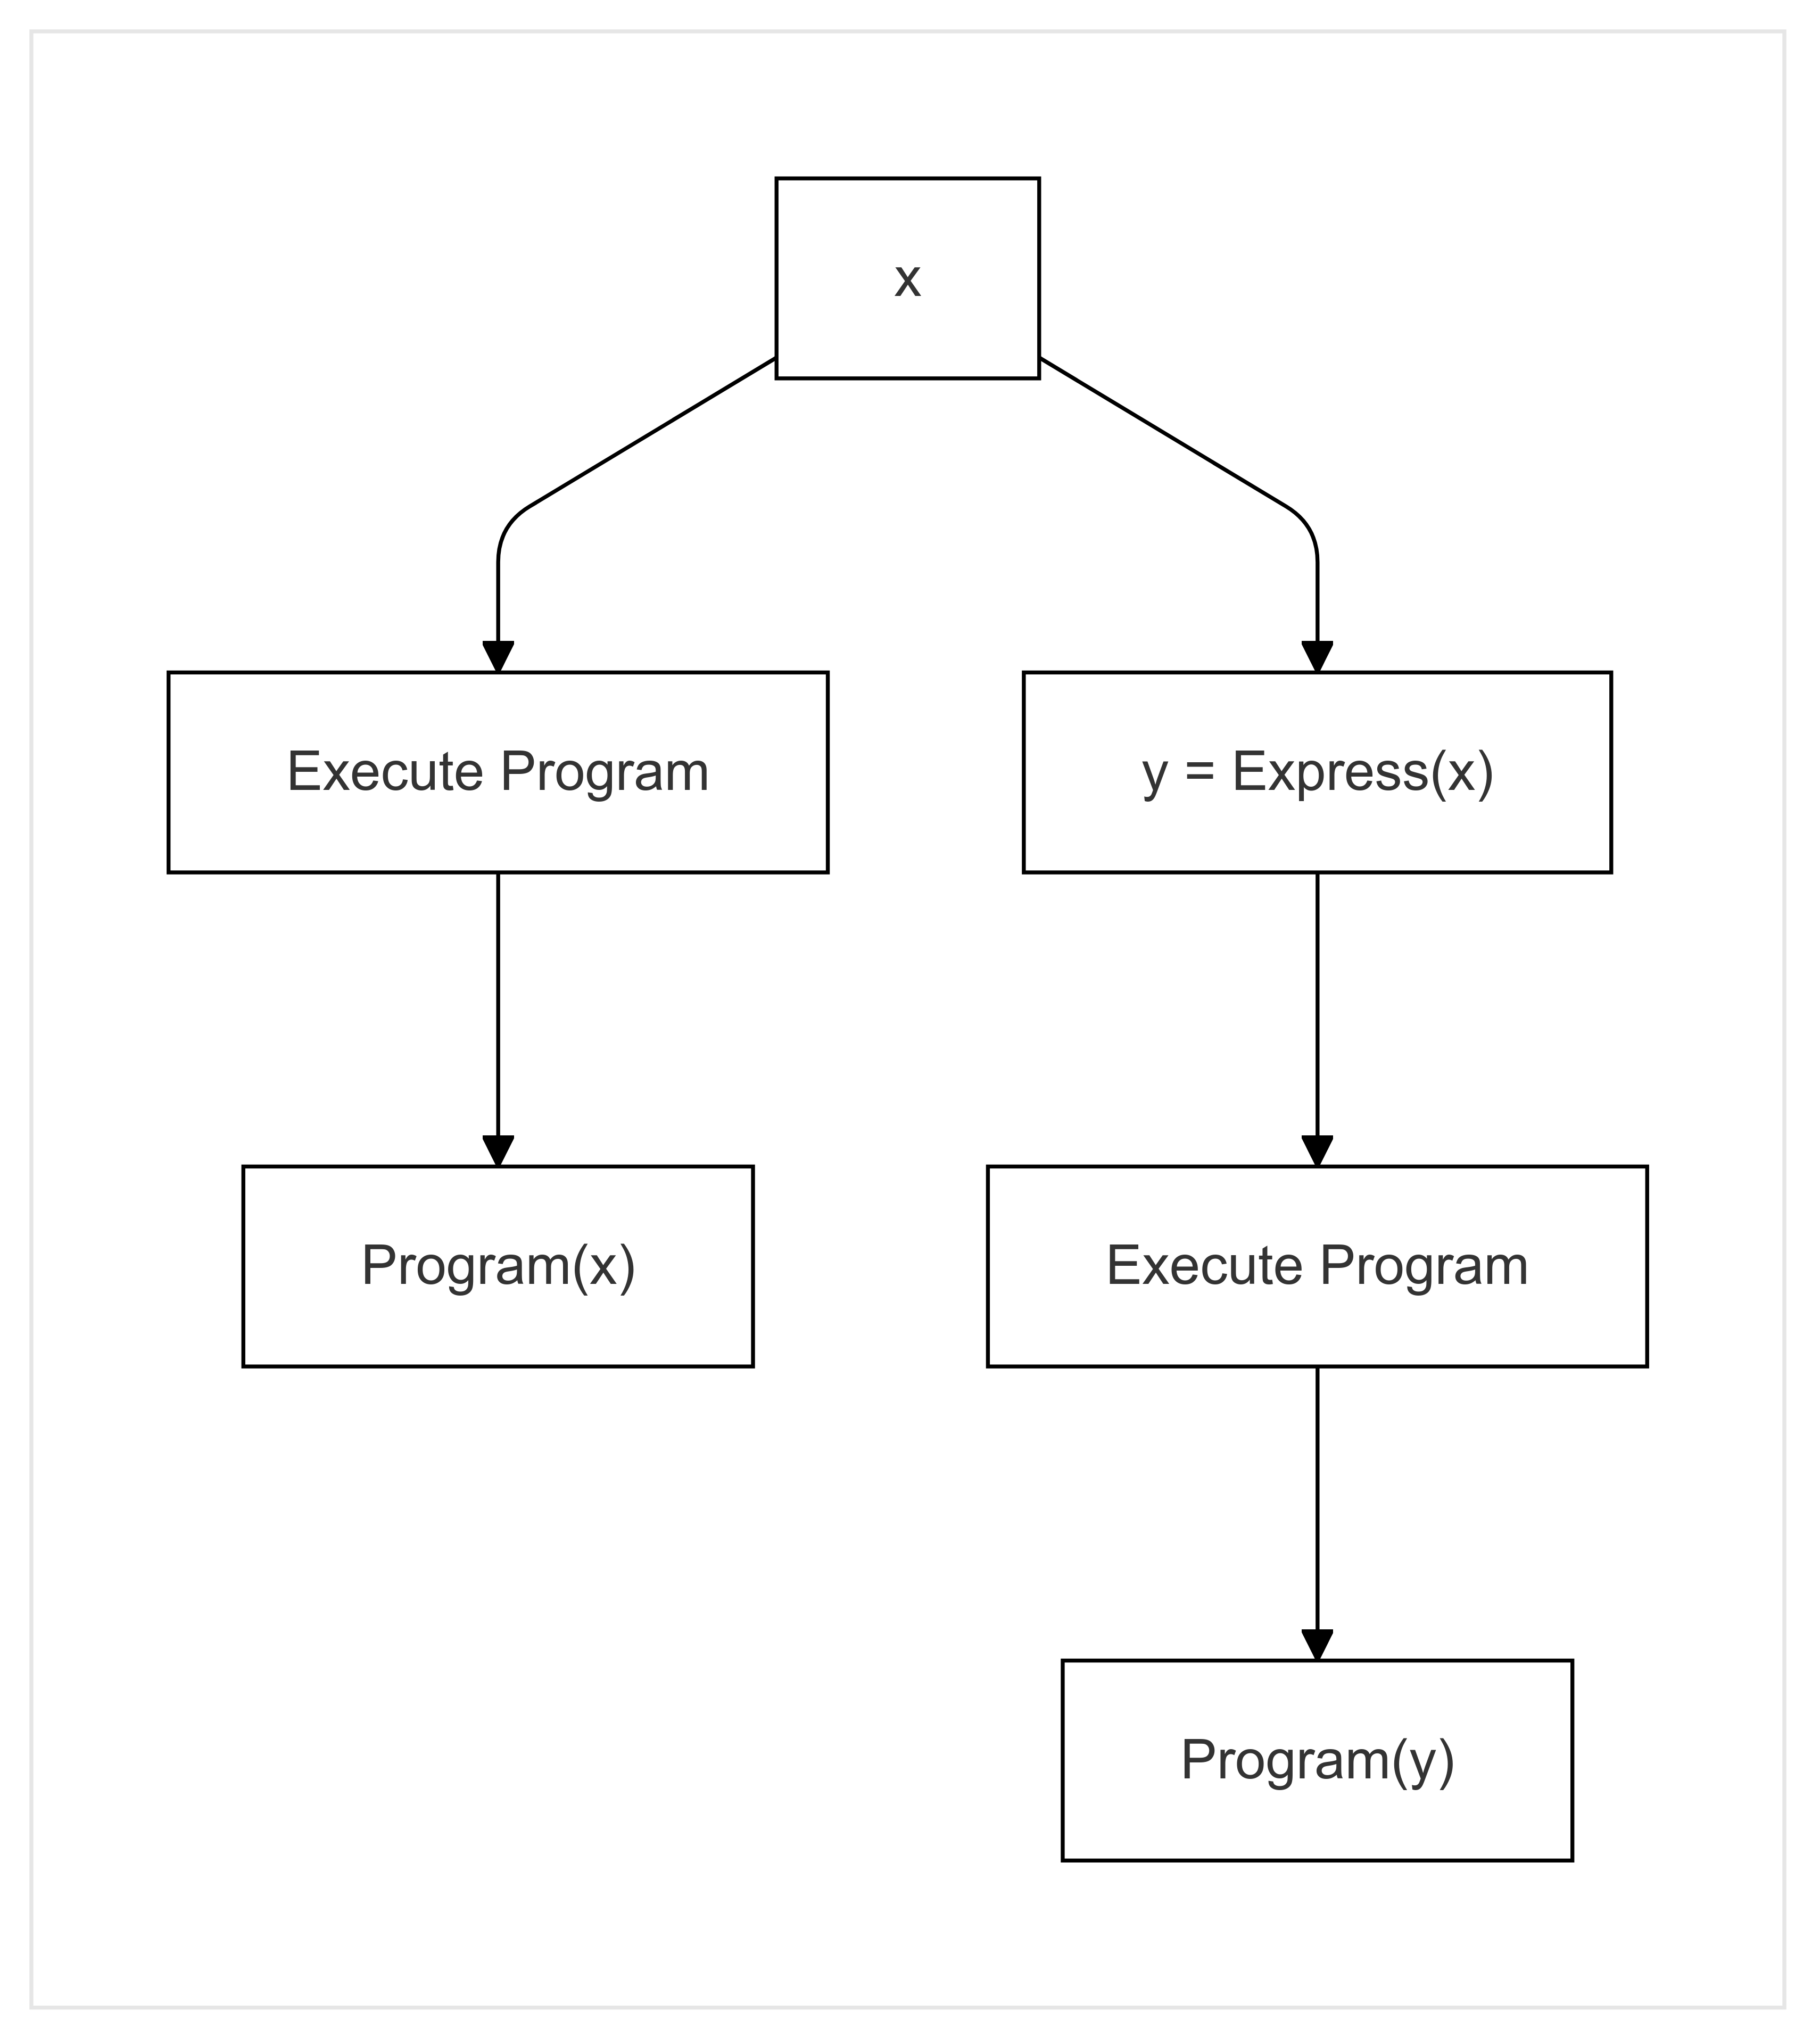
\includegraphics[width=0.7\textwidth]{diagrams/data_div/reexpress.png}
%     \caption{Data Reexpression}
%     \label{fig:data_rex}
% \end{figure}
\subsection{Previous work}

While the analysis so far was mostly theoretical, this section outlines methods already implemented and tested in practice, giving an insight into what we can expect when implemnting our own fault-tolerance methods.

\subsubsection{EDDI}

Error Detection by Duplicated Instructions \cite{eddi} (EDDI) is a pure software, technique that enhances runtime error detection by duplicating program instructions during compilation. Each original instruction (master instruction) is paired with a duplicate (shadow instruction) that operates on separate registers or variables. At key synchronization points, such as before memory writes or control transfers, the system compares the results of the master and shadow instructions. Any mismatch indicates an error, triggering a fault handler. EDDI leverages idle resources in super-scalar processors by interleaving these redundant instructions to maximize instruction-level parallelism while minimizing performance overhead. It is particularly effective in detecting transient faults, memory corruption, and control-flow deviations without requiring any hardware modifications, achieving over 98\% fault tolerance in benchmark programs.


\subsubsection{CFCSS}

Control Flow Checking by Software Signatures (CFCSS), originally proposed in \cite{994926} is a pure software method that embeds control-flow checking logic into a program at compile time. It is capable of detecting faulty branching or jumps within the program. 

The program is first divided into basic blocks, each representing a unique node in the control-flow graph. A unique signature is assigned to each node, and additional instructions are inserted to monitor the program's control flow during execution.

At runtime, the control flow is validated using a designated general-purpose register (GSR), which holds the expected signature. When control transfers to a new basic block, a new runtime signature is generated using a lightweight XOR-based function that combines the previous and current signatures. This updated signature is then compared with the expected one at the destination block. If a mismatch is detected, it indicates an illegal control transfer, and execution is redirected to an error handler.

CFCSS is particularly advantageous because it requires no dedicated hardware and can operate even in environments without multitasking support. Its effectiveness was validated through fault injection experiments, which showed that while 33.7\% of branching faults went undetected in unprotected programs, only 3.1\% remained undetected when CFCSS was applied, demonstrating an order-of-magnitude improvement in error detection coverage. CFCSS introduces moderate code size and execution time overhead (especially in branch-heavy programs).

\subsubsection{SWIFT}

SWIFT \cite{swift} (Software Implemented Fault Tolerance) is a compiler-based technique for detecting transient faults using software-only transformations, without requiring any specialized hardware. It builds upon earlier methods like EDDI by duplicating instructions and inserting validation checks, but improves upon them with several key optimizations to reduce memory and performance overhead. Unlike EDDI, SWIFT excludes memory from the sphere of replication, assuming protection is already provided by ECC in modern systems. It introduces an enhanced control-flow checking mechanism using software signatures, allowing it to detect illegal control transfers more reliably. Additionally, SWIFT incorporates optimizations such as restricting signature checks to store-containing blocks and eliminating redundant branch validation. These design decisions enable SWIFT to achieve high fault tolerance with lower execution and code size overhead. SWIFT demonstrated fault detection rates comparable to hardware-based methods while incurring significantly less overhead than previous software-only techniques.
\subsection{Chosen methods}

When considering the fault-tolerance methods to implement, the most crucial factor was the feasibility of implementation. Since we are working with a high-level language, certain methods such as EDDI are not possible to effectively implement, since they require implmenentation at assembly instruction level, however, modified or simplified version of these methods may still be implemented.

Ultimately, checkpoint and restart was chosen as the backbone of fault recovery, as it can be easily combined with other methods. CFCSS, with various modifications to make its implmentation feasible in Rust, was chosen to secure the control flow of the program. Finally, recovery blocks and N-version programming were chosen to facilitate multi-version functionality. Additional miscellaneous fault-tolerance methods were also used, such as variable protection through duplication to support the aforementioned methods.

\clearpage

\section{Motivation for Rust}
The secondary purposes of this thesis is to analyze the suitability of Rust language for the implementation of fault-tolerant software. Historically, C has been the most dominant language in this problem space, but Rust has numerous benefits which make it a strong candidate.

\subsection{Safe by design}
The goal of the Rust language is to eliminate the most common software bugs at the compiler level. An example of this is Rust's \textit{ownership and borrowing model} - a static code analysis done by the compiler \cite{rust_book:ownership}. It ensures memory safety of the program by explicity disallowing references to deallocated values, which prevents null pointer dereferencing, and also prevents race conditions by limiting the access to mutable variables. Rust's ownership model is a complex topic and explaning it in full is not within the scope of this thesis, more information can be found in the offical Rust book.

\subsection{Robust error handling}
Another major benefit of Rust is its approach to error handling. Rust splits errors into two categories: \textit{Unrecoverable} errors immediately terminate the execution of the program using the \textit{panic!()} macro and \textit{recoverable} errors which are return values of a function using the Result enum \cite{rust_book:error_handling}.

\begin{figure}[!h]
\begin{lstlisting}[language=Rust]
fn foo() -> Result<u32, ()> {
    ...
}
fn main() {
    let Ok(res) = foo() else {
        // Function returned with an error
    }
}
\end{lstlisting}
\caption{Rust - error as a value}
\label{fig:rust_error}
\end{figure}

Using the approach of \textit{error-as-a-value} we can determine if a function executed successfully by simply checking its return value (see figure \ref{fig:rust_error}). This can act as a very quick and rudimentary form of fault tolerance, since it can be easily applied to any function.

\subsection{Macro system}
Rust has a powerful macro system which in essence works as a code pre-processor acting over the abstract syntax tree. Unlike C macros, which only work as direct text replacement, Rust macros allow for arbitrary modification and generation of code before the compilation step. Using Rust macros, various fault tolerance techniques can be implmeneted. An example of utilizing macros is highlighted in this very thesis, where a Control Flow Checkign using Signature Streams (CFCSS) technique is implemented using Rust macro system. 

\subsection{Low-level control and C integration}
Rust demonstrates comparable functionality to C when it comes to low-level control - example being the ability to define custom heap allocator or the ability to use in-line assembly from within Rust. Since Rust uses LLVM under the hood, its compiler is able to link against existing C code. We can also easily use C functions within Rust by declaring the function signature (see figure \ref{fig:rust_extern}). This makes for an easy integration with existing C projects making Rust well suited as a higher level extension. This thesis demonstrates the use of Rust with FreeRTOS codebase written in C.

\begin{figure}[!h]
\begin{lstlisting}[language=Rust]
unsafe extern "C" {
    fn puts(string: *const c_char, len: usize) -> i32;
}
\end{lstlisting}
\caption{Rust - Using C function within Rust}
\label{fig:rust_extern}
\end{figure}

\newpage

\section{Environment}

This section outlines the implementation environment, including hardware constraints, system configuration, and software integration. It also describes key modifications made to support our specific use case.

\subsection{RISC-V}

The implementation was developed for a 32-bit RISC-V core, running in a simulated environment. The simulation features a single RAM region with a total size of 1MB. Of this, 8KB was allocated for the stack and another 8KB for heap memory. These parameters can be adjusted as needed for testing and experimentation.

A key feature of the RISC-V architecture is its interrupt and exception handling mechanism, which distinguishes between two primary types. \textit{Software exceptions} are triggered by the program itself, often to perform system calls, while \textit{hardware interrupts} are initiated by hardware events, such as timers or peripherals. The combination of these two systems allows for error detection and transferring control for recovery or rollback.

\subsection{FreeRTOS and Interrupt Management}

The system runs on the FreeRTOS kernel, a lightweight real-time operating system widely used in embedded systems. FreeRTOS is designed for minimal resource usage, making it suitable for constrained environments like our RISC-V simulation.

FreeRTOS uses \textit{tasks} to run user code. Task is a wrapper around user code which include the specific code's context. Tasks can be instantiated at any point during the program's lifetime. FreeRTOS \textit{scheduler} handles the execution of tasks as well as switching between them using the RISC-V hardware interrupt - \textit{Machine Timer Interrupt}.

In addition to timer-based preemption, FreeRTOS also makes use of software exceptions, such as those triggered by the RISC-V \textit{ecall} instruction. These interrupts are typically used for system-level operations and are routed, along with hardware interrupts, through a shared interrupt handler. In our case, this handler is implemented using a vectored interrupt table to efficiently dispatch control to the correct service routine.

\subsection{Rust Integration with FreeRTOS}

To enable Rust development on top of FreeRTOS, we used the open-source FreeRTOS-Rust library\footnote{\url{https://github.com/lobaro/FreeRTOS-rust}}. This library provides Rust bindings to the FreeRTOS C ABI. Modifications had to be done to ensure compatibility with our simulated environment. Notably, the used library required atomic instructions for certain functionality, however, our platform did not support atomic operations. Since we are only simulating single core, hardware multithreading is not a concern, as such, we could safely replace all atomic operations with their non-atomic counterparts.

On top of this, RISC-V Rust library\footnote{\url{https://github.com/rust-embedded/riscv}} was used to facilitate the compilation of Rust into a RISC-V acceptable binary. This library provided functionality such as designating the program entry point, designating the exception and interrupt handler functions and provided functions to work with RISC-V specific registers. However, the used library also added significant performance overhead in the form of BSS clearing segment before the main program start. Clearing BSS is useful to ensure all variables are initialized to 0 if a default value is not assigned. However, because Rust does not fundamentally allow for the use of non-instantiated variables this step was not necessary for our use case. By removing this segment we saved significant computation time, reducing the possible area for faults to manifest.
\clearpage

\clearpage
\section{Implementation}

The implementation section outlines some selected methods which were implemented using Rust and FreeRTOS and tested on a RISC-V core simulation. The implemented methods were modified to make them feasible to implement in a high level language.

\subsection{Checkpoint and restart}

Checkpoint and restart system is the backbone of our fault-tolernace framework, facilitating recovery. It can be used on its own to provide basic level of redundancy, or it can be combined with other techniques to boost their fualt-tolerance potential.

\subsubsection{Creating a checkpoint} \label{sec:creating_checkpoint}

\begin{figure}[!h]
\begin{lstlisting}[language=Rust]
asm!(
    // Storing registers in a static variable
    "lui   t0, %hi(CHECKPOINT)",
    "addi  t0, t0, %lo(CHECKPOINT)",
    "sw x1,   4(t0)",
    "sw x2,   8(t0)",
    ...
    "sw x31,124(t0)",
    "call set_checkpoint",
    // Restoring registers to their previous state
    "lui   t0, %hi(CHECKPOINT)",
    "addi  t0, t0, %lo(CHECKPOINT)",
    "lw x1,   4(t0)",
    "lw x2,   8(t0)",
    ...
    "lw x31,124(t0)",
)
\end{lstlisting}
\caption{Rust - Creating checkpoint}
\label{fig:rust_create_checkpoint}
\end{figure}

Checkpoint is generated by creating a \textit{checkpoint context} during which the current state of the application is stored. Namely, the general purpose registers (x1 - x31 in RISC-V 32bit) are stored into a static memory location before the execution of a \textit{checkpoint block} (the part of code protected by the checkpoint). Additionally, a return address is stored along with the general purpose registers. 

Higher-level programming languages do not directly provide the functionality to manipulate register values. This means assembly instructions have to be used to facilitate the low level access as seen in figure \ref{fig:rust_create_checkpoint}.

In order to set the return address, we utilize a trick (shown in figure \ref{fig:rust_set_checkpoint}) whereby calling a function we now have access to the instruction immediatelly following the function call (figure \ref{fig:rust_create_checkpoint} line 11) saved in the return address register (RA). We store the value of this register along with the registers in the checkpoint variable.

\begin{figure}[!h]
\begin{lstlisting}[language=Rust]
fn set_checkpoint() {
    unsafe {
        asm!(
            "sw ra, ({0})",
            in(reg) &(CHECKPOINT.ret_addr),
        );
    }
}
\end{lstlisting}
\caption{Rust - Set checkpoint}
\label{fig:rust_set_checkpoint}
\end{figure}

\subsubsection{Storing the checkpoint}

As mentioned in section \ref{sec:creating_checkpoint}, the checkpoint information is stored in a static memory location. This might seem as an arbitrary decision given that storing the checkpoint on the stack or the heap are also an option. Each of the listed approaches comes with its own issues. Using a static memory location limits the number of checkpoints that can be stored. Using the stack for checkpoint storage can be very unreliable as stack corruption can easily occur should the stack pointer manifest a fault. And using the heap is generally slow and prone to error stemming from pointer corruption or premature memory freeing which could occur in the prsence of faults.

Our implementation uses a hybrid approach of using a static memory location for the storage of the \textit{primary checkpoint} (the last checkpoint that was set), while pushing any older checkpoints on the stack. This heightens the chance that at least the primary checkpoint will be available. Once the primary checkpoint context ends, the previous checkpoint is popped from the stack and can be used again. This allows for infite nesting of checkpoints, provided we have enough memory.

\subsubsection{Returning to the checkpoint}

After setting the checkpoint, the program execution continues as per usual, until either the checkpoint block finishes successfuly, or an error is detected. An error can be detected in two way, an exception is detected by the processor, or an error is detected via checks inserted into the checkpoint block.

If the processor detects an error the exception handler subroutine is called. We can hook into this subroutine and use it to restore the stack pointer to the pre-checkpoint block state and then perform a jump back to the saved return address.

If an error is detected via checks inserted by the programmer, checkpoint restart can be triggered by simply returning an error (Err()) from within the checkpoint block.

Both forms of error detection and returning to checkpoint result in the restoration of the program context to the program state in which the checkpoint function was called. After the context was restored, checkpoint block will be attempted again if retries are allowed, otherwise the entire checkpoint context returns an erroneous value.

\begin{figure}[!h]
\begin{lstlisting}[language=Rust]
if let Err(Error::MaxRetriesReached(n)) = checkpoint(2, || {
    // Checkpoint block here
    ...
    Ok(())
}) {
    println(&format!("Max retries reached: {}", n));
}
\end{lstlisting}
\caption{Rust - Using the checkpoint system}
\label{fig:rust_using_checkpoint}
\end{figure}

\subsubsection{Overhead}

The implemented checkpoint system incurs minimal instruction overhead. Additional instructions are only inserted when creating the checkpoint context and just before the end of the checkpoint context. This comes out to 79 additional instructions to save and restore program state, plus approximately 300 instructions to save and restore old checkpoint and perform various error checks, without factoring in any compiler optimizations.

This overhead is constant for the entire checkpoint block, irrespective of the checkpoint block size. As such, the ratio of overhead instructions to the checkpoint block instructions is solely determined by the size of the protected checkpoint block.

\subsubsection{Considerations} \label{sec:checkpoint_considerations}

Checkpoint system only facilitates basic restart and retry functionality. It can be used on its own when only basic level of protection is required, however, in most cases, checkpoint and restart system is meant to be used as a framework to build upon. Namely, the multi-version techniques outlined in later sections all use checkpoints to implement version switching.

Our implmenetation of the checkpoint and restart system only saves the minimal required state, which in the case of RISC-V, is the general registers. This limits the use of the checkpoint system as other memory regions such as stack or heap are not stored. Careful consideration needs to be given to the code block protected by the checkpoint context. If the checkpoint body has any side-effects, such as modifying global variables, variables outside of the checkpoint block scope or writing to heap, these alterations will not be reversed in the case of an error and subsequent checkpoint return.

This problem can be avoided by explicitly creating a copy of any outside variable which needs to be modified within the checkpoint block. The copy will then be used within the checkpoint block and the original variable will only be overrided if the checkpoint context returns successfully. More on this in section \ref{sec:var_protection}.

Another important thing to mention is that our implementation does not save registers other than the general purpose registers. This means special registers such as \textit{mtvec}, \textit{mcause} or \textit{mstatus} are not protected by the checkpoint system. The fault-insertion simulation does not insert faults into these registers, as such their directly protection is not needed. However, errors can still manifest (as if they occuerd in the special registers) in ALU after the special registers are read for processing.

\clearpage

\subsection{CFCSS}

Unlike the usual implementation, which works over assembly instructions, or LLVM's intermediate representation (IR), our implementation takes advantage of Rust's macro system to insert CFCSS directly into program code. An algorithm originally designed for LLVM IR is used, with modifications to make it suitable for our purposes \cite{coast:cfcss}.

Macro is used to designate a \textit{module} as CFCSS protected, each function within the module being designated as a \textit{block} ({$b_n$}). A graph is then generated at compile time representing the allowed control flow within the protected module. Each block within the graph is assigned a random unique signature ({$s_n$}) and signature difference ({$d_n$}), which is calculated by XORing ({$\oplus$}) the current block's signature and the signature of its predecessor as seen in equation \ref{eq:block_diff}.

\begin{equation}
d_n = s_n \oplus s_{n-1}
\label{eq:block_diff}
\end{equation}

\begin{figure}[!h]
    \centering
    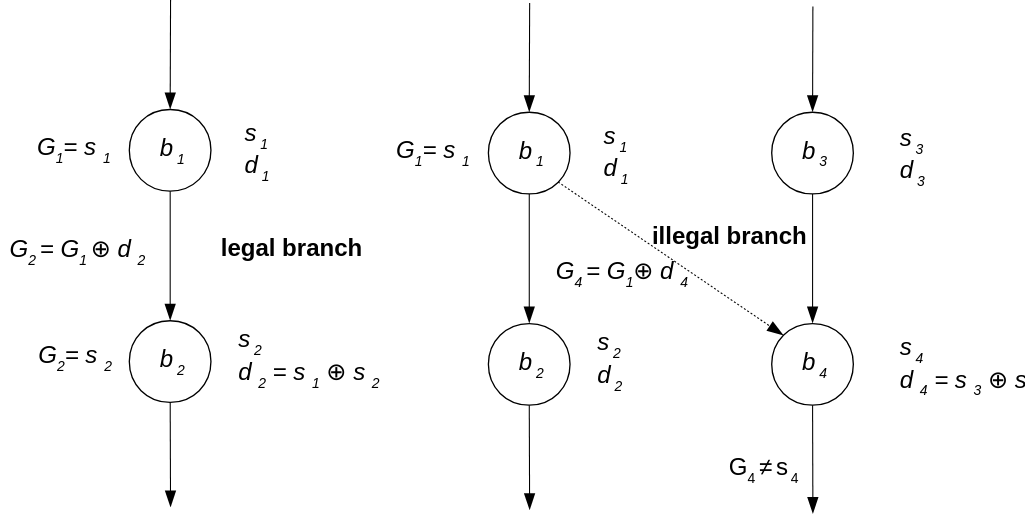
\includegraphics[width=1.0\textwidth]{diagrams/cfcss/basic.png}
    \caption{Basic CFCSS \cite{coast:cfcss}}
\end{figure}

A runtime signature {$G_n$} is also created for the given protected module, initially set to {$G_0 = 0$}. This signature is updated at runtime before the execution of every block by XORing it with the signature difference of the destination block (equation \ref{eq:runtime_sig}). Using XOR to update the runtime signature is favorable, since XOR operation can be undone by simply being repeated, which is desirable when returning from a block.

\begin{equation}
\label{eq:runtime_sig}
G_n = G_{n-1} \oplus d_n
\end{equation}

To ensure correct control flow, the newly calculated runtime signature must be equal to the function signature, otherwise an invalid branching occured.

\begin{equation}
\label{eq:sig_check}
G_n = s_n
\end{equation}

This approach is, however, insufficient in the presence of so-called \textit{fan-in} block. If both {$b_1$} and {$b_3$} have an edge to {$b_4$} a problem arises where (provided that {$s_1 \ne s_3$}) either {$G_4 = G_1 \oplus d_4$} is true or {$G_4 = G_3 \oplus d_4$}.

\begin{figure}[!h]
    \centering
    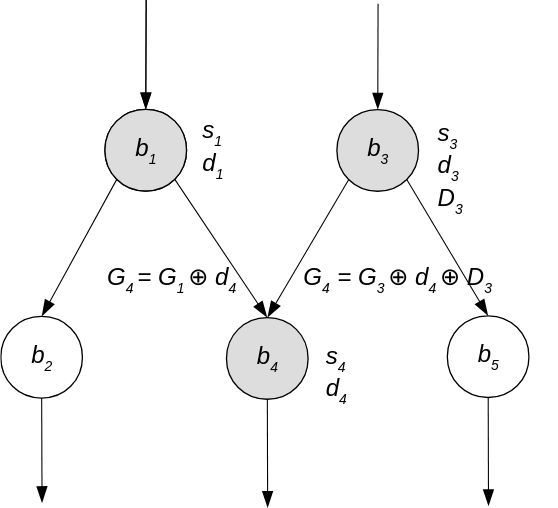
\includegraphics[width=0.6\textwidth]{diagrams/cfcss/adjuster.png}
    \caption{CFCSS with fan-in block \cite{coast:cfcss}}
\end{figure}

We need to introduce another constant called signature adjuster ({$D_n$}) caluclated for each predecessor of a fan-in node, and apply it while updating the runtime signature. This gives us the actual equation (\ref{eq:runtime_sig_with_adj}) for updating runtime signature.

\begin{equation}
\label{eq:runtime_sig_with_adj}
G_n = G_{n-1} \oplus d_n \oplus D_n
\end{equation}

\subsubsection{Macro implementation}

The Rust macro generates static variables ({$G_n, D_n, s_n, d_n$}) during compile time and inserts additional code before and after the actual function code witin the protected module (see figure \ref{fig:rust_cfcss_macro}). The instructions inserted after the function block are equivalent to the ones inserted before, with the exception of restoring \textit{last adjuster} from stack instead of updating and storing it.

\begin{figure}[!h]
    \begin{lstlisting}[language=Rust]
    RUNTIME_SIGNATURE ^= #dif_name;
    if is_fan_in {
        RUNTIME_SIGNATURE ^= RUNTIME_ADJUSTER;
    }
    if #sig_name != RUNTIME_SIGNATURE {
        return_to_checkpoint(ERROR_MSG);
    }
    if func_has_adjuster {
        RUNTIME_ADJUSTER = #adj_name;
    }
    \end{lstlisting}
    \caption{Rust - CFCSS instructions inserted before function block}
    \label{fig:rust_cfcss_macro}
    \end{figure}

This macro can be applied as shown in figure \ref{fig:rust_cfcss_macro_example} by specifying a module as \textit{\#[cfcss\_root]}. An entry funciton is designated with a special macro \textit{\#[entry]}, this macro embeds additional instruction that reset the runtime signature and adjuster of the module, allowing for repeated call of the entry point. An entry function can only be a function that is not called from within another function in the protected module.

\begin{figure}[!h]
\begin{lstlisting}[language=Rust]
#[cfcss_root]
pub mod protected_block {
    fn function_0();
    fn function_1();
    #[entry]
    pub fn entry_function() {
        function_0();
        function_1();
    }
}
\end{lstlisting}
\caption{Rust - Using the CFCSS macro}
\label{fig:rust_cfcss_macro_example}
\end{figure}

\subsubsection{Overhead}

Embedding new instruction during compile time will understandably have performance impact on the execution of the program. Each function will incur a execution overhead, as multiple operations and checks must be carried out before the actual function body executes. Approximately 50 additional assembly instructions are inserted before the function block and 50 more after the function block, without using any compiler optimizations.

However, due to the nature of the implementation, the developer is in full control of just how much overhead is incurred. Since the number of additional instructions is constant per function definition, we can either split our protected module into fewer function to have less overhead, but at the cost of less fault-tolerance. Or we can fragment our code into as many function blocks as possible, and thereby increasing the number of control flow checks performed.

\subsubsection{Considerations}

Since our implementation of CFCSS utilizes a purely code based approach it natuarally comes with several limitations. Unlike the traditional approach, which implements CFCSS at IR level by extending the LLVM pipeline we do not have access to the underlying instructions, which limits the possible density of the control flow checks. An IR approach is able to precisely insert instructions after every branch and jump operations, and also has more granular control over the actual instructions being inserted. This means our implementation is more prone to control flow errors. Although not within the extent of this thesis, further improvements could be made by directly extending Rust's LLVM pipeline and integrating a CFCSS method at IR level.

Additionally, CFCSS is incompatible with the aforementioned checkpoint and restart system. As explained in section \ref{sec:checkpoint_considerations}, our checkpoint and restart system does not restore context of static variables, which CFCSS relies on for proper functioning. As such, checkpoints cannot be used within a CFCSS protected module, since if a checkpoint restart were to happen, the runtime signature and adjuster would not be reset to their proper pre-checkpoint values.
\clearpage

\subsection{Protection of variables} \label{sec:var_protection}

Various unforeseeable circumstances can lead to the corruption of program variables, from direct corruption of registers storing the variables to indirect side-effect originating from errors within function that work with said variables. This section focuses on various techniques implemented to ensure the reliability of critical program variables with varying degree of protection depending on the use case.

\subsubsection{Copy and commit}

Copy and commit is a method inspired by a common practice in database transaction handling, where a temporary copy of the variable is created and modified instead of the original value. Upon an explicit commit, the original variable is overwritten with the modified copy. This pattern resembles \textit{libft} \cite{libft} variable protection and is particularly useful in combination with checkpoint and restart to avoid unintended side-effects. In the Rust example shown in Figure~\ref{fig:rust_copy_commit}, a CopyCommit wrapper is used to hold a temporary copy of the value. Inside the bar function, the value is incremented, but the change only takes effect on the original data when commit() is called. This allows for greater control over when and how mutations are finalized.

\begin{figure}[!h]
\begin{lstlisting}[language=Rust]
fn bar(mut a: CopyCommit<u32>) {
    *a += 1;
    a.commit();
}

fn foo() {
    let mut a = 1;
    bar(CopyCommit::new(&mut a));
}
\end{lstlisting}
\caption{Rust - Copy and commit example}
\label{fig:rust_copy_commit}
\end{figure}

While this method gives us more control over when variables are modified and helps prevent unwanted side-effects, it inherently does not provide any fault tolerance against direct corruption of variables. As such, it should only be reserved for non-critical parts of the program, and or combined with other variable protection techniques.

\subsubsection{Multiple redundant variables}

Another way we can secure a variable is creating multiple copies of it and applying any modification to all the copies. The modified copies are then compared against each other to detect any mismatch. With two copies of a variable, we can detect an error but cannot correct it, since we cannot tell which one of the copies is faulty. With three copies, we can detect an error but also perform correction, if at least two copies of the variable are equal. The more copies we create the more likely we are to have a majority of the variables be equal, therefore the more confident we can be in our fault-tolerance.

\begin{figure}[!h]
\begin{lstlisting}[language=Rust]
// Creates 3 identical copies
let mut a = MultiVar::new(0);

// Applies the edit function to each of the copies and performs equality check
if let Err(e) = a.edit(|ptr_a| {
    *ptr_a += 1;
}) {
    // Error while updating variable
    ...
}
\end{lstlisting}
\caption{Rust - Multiple variable redundancy}
\label{fig:multivar}
\end{figure}

In our implementation, a MultiVar wrapper around a variable is used to automatically instantiate three separate copies of the variable as seen in Figure \ref{fig:multivar}. By calling the edit function on the wrapper, we map any modification to all the copies of the variable. The edit function also includes an internal checks which tries to correct the variables in a case of a mismatch. If correction is not possible this function returns an error.

\subsubsection{Checksum} \label{sec:checksum}

Checksum is a technique to ensure a long-lived variable has not been corrupted during the execution of the program. If we need to store a variable for prolonged amount of time we can store a checksum along with it. The checksum is calculated by splitting the stored data into chunks of 32-bits each and XORing these chunks with one another, thereby generating an unique signature.

Every time the protected variable is modified the checksum is updated by recalculating the signature. Before the variable data is read again at a later point in the program, a checksum is recalculated and compared with the stored checksum. If the checksums match the variable has not been changed since the last proper modification. In the case of a checksum mismatch, however, the variable is likely to have been unexpected modified or directly corrupted.

This technique is best utilized for global variables, since they live for the duration of the program and their correctness is paramount for the proper application functioning.

\subsubsection{Considerations}

The implemented methods for variable protection can give us more confidence in the correctness of the program variables, however, no matter the degree of protection and fault-tolerance implemented, faults can always manifest. Since data corruption can happen on the ALU directly, even if our stored variable is correct, the actual value being read and processed by the CPU can appear to be faulty. As such, the methods listed above are not sufficient on their own to ensure we get the correct result even if the program executes without any errors detected.

\clearpage

\subsection{Multiversion}

The implemented multiversion techniques are clumination of most of the techniques discuessed so far.

\subsubsection{Recovery blocks}

Recover blocks have been implemented by taking advantage of the checkpoint system. By wrapping each call to a different version function in a checkpoint context we ensure that the function will return even in case of an error. We can then check the return value of the checkpoint block to determine if the version executed successfully. As seen in Figure \ref{fig:recover_blocks}, if the version returns successfully, we immediatelly return the value, otherwise we try another version. The checkpoint is set to 0 retries, meaning each one of the versions (fib\_v1, fib\_v2, fib\_v3) will only be tried once.

\begin{figure}[!h]
\begin{lstlisting}[language=Rust]
pub fn fib_rec_blocks(x: u8) -> Result<u32, &'static str> {
    // Version 1
    if let Ok(res) = checkpoint(0, || fib_v1(x)) {
        return Ok(res);
    }
    // Version 2
    if let Ok(res) = checkpoint(0, || fib_v2(x)) {
        return Ok(res);
    }
    // Version 3
    if let Ok(res) = checkpoint(0, || fib_v3(x)) {
        return Ok(res);
    }
    Err("Versions exhausted")
}
\end{lstlisting}
\caption{Rust - Recovery blocks}
\label{fig:recover_blocks}
\end{figure}

Important thing to mention is the lack of any verification of the result. In the case of recovery blocks, we only care about the function executing without obvious errors. The return value could be corrupted by an undetectable bit flip somewhere in the function variables. Recovery blocks alone does not deal with this issue.

\clearpage
\section{Testing}

Testing of the implementation was done on Hardisc\footnote{\url{https://github.com/janomach/the-hardisc}} (simulated using ModelSim) - a hardened RISC-V core with the ability to statically insert faults during runtime of the program. The form of the fault is a single bit-flip. The \acrfull{fi} was delayed by approximately 36 000 CPU cycles to give FreeRTOS enough time to initialize, after which point one fault was inserted approximately every 2500 CPU cycles. Depending on the duration of the benchmark, up to 100 faults could be inserted per benchmark. For the purpose of narrowing down the scope of the thesis, faults were only inserted in the general purpose registers and the execution pipeline (\acrshort{rfc}, \acrshort{alu}, \acrshort{mdu}, \acrshort{dp}, \acrshort{tp}).

Notably, \acrfull{ram} was exempt from \acrshort{fi}s during our testing. Should a non-transient error occur in the part of \acrshort{ram} which holds the program instructions there would be no way to properly recover from it using software-only fault tolerance. Usually, \acrshort{ram} and CPU duplication is used, effectively running the same program twice in parallel with set synchronization points. This method is outside of the scope of software implemented fault tolerance.

The methods outlined in the implementation section, however, are in theory capable of detecting and recovering from certain faults in \acrshort{ram}. As mentioned in section \ref{sec:checksum}, checksums are capable of detecting corruption in variables, this includes variables stored in the \acrshort{ram}. Similarly, using multiversion programming can provide tolerance even in the case of non-transient error occurring in one of the versions. Due to general unreliability of this approach, however, the testing on \acrshort{ram} \acrshort{fi}s was not conducted.

\subsection{Benchmarks}

A set of benchmarks was selected to evaluate the effectiveness of the implemented fault tolerance techniques. These benchmarks primarily consist of common arithmetic operations and data manipulation tasks representative of typical embedded system workloads. 

In addition to standard benchmarks, one unique benchmark - \textit{Nested Function Calls} (NFC) was included. This benchmark involves a series of functions invoking one another in a nested manner, creating intertwined control-flow graph. It was specifically chosen to assess the performance impact of \acrshort{cfcss}, which is particularly sensitive to complex function call hierarchies.

Benchmark programs report results in one of two ways, successful execution (0) and unrecoverable error (1). Any other return status code is considered an unknown error. The reliability of the fault tolerance was measured as a sum of successful executions and correctly reported unrecoverable errors divided by the overall number of executions (25 per benchmark). Each benchmark was given equal amount of time to execute (100 000 CPU cycles), if the time threshold is reached the program ends in a timeout. Notably, a timeout does not necessarily mean the benchmark itself did not execute correctly. It is very common for the FreeRTOS scheduler to be the source of an error leading to a timeout. FreeRTOS can take upwards of 10 000 CPU cycles to initialize the scheduler and being the execution of the first task. During this time window, the program is exceptionally prone to faults resulting in unrecoverable errors, as our implemented fault tolerance approach does not directly modify the FreeRTOS codebase or instructions being executed. As such, in the case of a timeout, the output logs are examined to determine if the benchmark succeeded.

\begin{table}[h]
\centering
% \resizebox{\linewidth}{!}{%
\begin{tabular}{|l|c|c|c|c|}
\hline
\textbf{Fib sequence} & \textbf{Correct} & \textbf{Errors Reported} & \textbf{Timeouts} \\
\hline
Unprotected & 10 & 5 & 8 \\
Protected & 14 & 9 & 3 \\
\hline
\end{tabular}
% }
\caption{Fibonacci sequence benchmark statistics}
\label{tab:fib_bench}
\end{table}

As seen in Table \ref{tab:fib_bench} the overall fault detection of the protected benchmark went up significantly. The increase in correct results was not exceptionally high, likely due to the fact that errors mostly occurred outside of the variables and registers that would directly alter the computation result. Rather, most faults resulted in errors manifesting in various supporting subroutines. Evidence of this is the nearly doubled number of reported errors when fault tolerance was enabled.

\begin{table}[h]
\centering
% \resizebox{\linewidth}{!}{%
\begin{tabular}{|l|c|c|c|c|}
\hline
\textbf{Matrix dot product} & \textbf{Correct} & \textbf{Errors Reported} & \textbf{Timeouts} \\
\hline
Unprotected & 16 & 0 & 9 \\
Protected & 18 & 7 & 0 \\
\hline
\end{tabular}
% }
\caption{Matrix dot product benchmark statistics}
\label{tab:matrix_bench}
\end{table}

Similar trend can be observed in the case of Matrix benchmark (see Table \ref{tab:matrix_bench}). The correct results difference is even lower, likely due to the fact that the matrix dot product test requires less CPU instructions, and therefore is a relatively smaller time window for faults to manifest. However, the overall error reporting went up significantly, proving our fault detection methods are good at catching error that would otherwise result in unexpected program termination.

\begin{table}[h]
\centering
% \resizebox{\linewidth}{!}{%
\begin{tabular}{|l|c|c|c|c|}
\hline
\textbf{Bubblesort} & \textbf{Correct} & \textbf{Errors Reported} & \textbf{Timeouts} \\
\hline
Unprotected & 15 & 2 & 8 \\
Protected & 18 & 7 & 0 \\
\hline
\end{tabular}
% }
\caption{Bubblesort benchmark statistics}
\label{tab:bubblesort_bench}
\end{table}

Bubblesort benchmark also matches the previous observations. It further confirms that while our implementation only has marginal impact on the correctness of the result, the overall fault detection and ability to avoid timeouts is greatly improved with protection enabled.

\subsection{Testing with delayed FI}

As previously mentioned, the initial startup of FreeRTOS scheduler took up a significant portion of the program runtime. During initialization, only basic fault tolerance is possible without directly modifying FreeROTS source code. For that reason, we also attempted a single round of testing with unprotected scheduler and delayed FI to give FreeRTOS enough time to initialize, before starting fault insertion. This ensures faults would only occur in the part of program directly under our control.

For this specific test, we also lowered the FI saturation down to one fault every 4000 CPU cycles. To ensure faults would still affect our tests, the benchmark was adjusted to take more time, by increasing the Fibonacci number being computed. We executed the benchmark 100 times, with an equal split between protected and unprotected variants.

The findings from this test can be seen in Fig. \ref{tab:fib50_delayed}. The rate of timeout and unexpected program terminations became roughly equivalent, reinforcing our suspicion that timeouts mostly occur as a result of fault manifesting in the scheduler subroutines. The rate of successful executions, however, rose up significantly in the protected benchmark - 47.82\% increase over the unprotected benchmark, compared to the increase of approx. 20\% in the benchmarks without FI delay. This further solidifies the claim that our fault tolerance methods can increase the success rate of the program.

\begin{table}[h]
\centering
% \resizebox{\linewidth}{!}{%
\begin{tabular}{|l|c|c|c|c|}
\hline
\textbf{Fibonacci (FI Delay)} & \textbf{Correct} & \textbf{Errors Reported} & \textbf{Timeouts} \\
\hline
Unprotected & 23 & 17 & 4 \\
Protected & 34 & 8 & 5 \\
\hline
\end{tabular}
% }
\caption{Fibonacci benchmark with delayed FI}
\label{tab:fib50_delayed}
\end{table}

\subsection{Performance impact}

Performance impact of the implemented fault-tolerance methods was measured without employing any compiler optimizations on a fault-free version of the simulated core. In the presence of faults, the effective performance could vary unexpected, influenced by the randomness of the \acrshort{fi}. As such, there is not much point in measuring performance in the presence of faults.

The test were measured in CPU cycles using the RISC-V \textit{mcycle} and \textit{mcycleh} registers.

\begin{table}[h]
\centering
\resizebox{\linewidth}{!}{%
\begin{tabular}{|l|c|c|c|}
\hline
\textbf{Test} & \textbf{Unprotected (cycles)} & \textbf{Protected (cycles)} & \textbf{Increase (\%)} \\
\hline
Fibonacci & 30734 & 34983 & 13.82\% \\
Matrix & 9871 & 11133 & 12.78\% \\
NFC & 9889 & 13126 & 32.73\% \\
Bubblesort & 15228 & 16773 & 10.14\% \\
CRC & 8278 & 10614 & 28.21\% \\
\hline
\end{tabular}
}
\caption{Execution time comparison between unprotected and protected tests}
\label{tab:time_increase}
\end{table}

As expected, looking at Table \ref{tab:time_increase} we see an increase in CPU cycles it takes to execute the protected version as opposed to the unprotected one. Fibonacci, Matrix and Bubblesort (group one) test only incurred roughly 12\% increase, while both NFC and CRC (group two) incurred much more substantial increase. The main difference between these two groups of tests is their flow graph complexity. Group one has linear control flow and mostly consists of 1-4 function call, meaning very little time is spent on \acrshort{cfcss} checking. Group two has more complex control flow resulting in a lot of \acrshort{cfcss} checks.

% Comparing the results of select tests without CFCSS (Table \ref{tab:cfcss_nocfcss}), we can deduce several things. The additional CPU cycles needed for checkpoint and multiversion protection is between 1000 and 1500 cycles. This is a constant increase and should not scale with the control flow complexity or instruction size of the tests. The CFCSS 

% \begin{table}[h]
% \centering
% % \resizebox{\linewidth}{!}{%
% \begin{tabular}{|l|c|c|}
% \hline
% \textbf{Test} & \textbf{With CFCSS} & \textbf{Without CFCSS} \\
% \hline
% Fibonacci sequence & 34983 & 31881 \\
% Nested function calls & 13126 & 11828 \\
% CRC calculation & 10614 & 8746 \\

% \hline
% \end{tabular}
% % }
% \caption{Protected fibonacci test with and without CFCSS}
% \label{tab:cfcss_nocfcss}
% \end{table}

\subsection{Size impact \& compiler optimizations}

To evaluate the memory overhead introduced by the fault tolerance mechanisms, we compared the size of the compiled binaries with and without protection under two conditions: with no compiler optimizations and with standard Rust \textit{release profile} optimizations enabled, more details on the used optimizations can be found in the official Rust book\footnote{\url{https://doc.rust-lang.org/cargo/reference/profiles.html}}. As expected, enabling protection introduces additional instructions and data structures, resulting in larger binary sizes. The impact is more pronounced in the unoptimized build, while optimized builds show a more moderate increase due to compiler optimizations reducing overall code size.

\begin{table}[!h]
\centering
\begin{tabular}{|l|c|c|c|}
\hline
\textbf{Compiler optimizations?} & \textbf{Unprotected} & \textbf{Protected} & \textbf{Size increase} \\
\hline
NO  & 23164 & 32847 & 41.8\% \\
YES & 8467 & 9216 & 8.84\% \\
\hline
\end{tabular}
\caption{Binary size increase with and without protection}
\end{table}

However, using the compiler optimizations comes with some risks. When examining the performance of select compiler optimized benchmarks, fault tolerance was noticeably lacking. Upon examining the compiled binary, it was determined that the compiler optimizations reorganized the order of some instruction blocks, effectively negating the effects of the implemented fault tolerance. Compiler optimizations make it harder to reason about the final form of the compiled binary, making them possibly unsuitable for fault tolerant software.


\clearpage
\section{Conclusion}


\clearpage
\section{Resumé}

\newpage
\printbibliography

\end{document}

